% Template for Elsevier CRC journal article
% version 1.2 dated 09 May 2011

% This file (c) 2009-2011 Elsevier Ltd.  Modifications may be freely made,
% provided the edited file is saved under a different name

% This file contains modifications for Procedia Computer Science
% but may easily be adapted to other journals

% Changes since version 1.1
% - added "procedia" option compliant with ecrc.sty version 1.2a
%   (makes the layout approximately the same as the Word CRC template)
% - added example for generating copyright line in abstract

%-----------------------------------------------------------------------------------

%% This template uses the elsarticle.cls document class and the extension package ecrc.sty
%% For full documentation on usage of elsarticle.cls, consult the documentation "elsdoc.pdf"
%% Further resources available at http://www.elsevier.com/latex

%-----------------------------------------------------------------------------------

%%%%%%%%%%%%%%%%%%%%%%%%%%%%%%%%%%%%%%%%%%%%%%%%%%%%%%%%%%%%%%
%%%%%%%%%%%%%%%%%%%%%%%%%%%%%%%%%%%%%%%%%%%%%%%%%%%%%%%%%%%%%%
%%                                                          %%
%% Important note on usage                                  %%
%% -----------------------                                  %%
%% This file should normally be compiled with PDFLaTeX      %%
%% Using standard LaTeX should work but may produce clashes %%
%%                                                          %%
%%%%%%%%%%%%%%%%%%%%%%%%%%%%%%%%%%%%%%%%%%%%%%%%%%%%%%%%%%%%%%
%%%%%%%%%%%%%%%%%%%%%%%%%%%%%%%%%%%%%%%%%%%%%%%%%%%%%%%%%%%%%%

%% The '3p' and 'times' class options of elsarticle are used for Elsevier CRC
%% Add the 'procedia' option to approximate to the Word template
%\documentclass[3p,times,procedia]{elsarticle}
\documentclass[3p,times]{elsarticle}

\usepackage{soul}
\usepackage{url}
\usepackage[utf8]{inputenc}
\usepackage{caption}
\usepackage{graphicx}
\usepackage{amsmath}
\usepackage{amsthm}
\usepackage{booktabs}
\usepackage{algorithm}
\usepackage{algpseudocode}
\usepackage{appendix}
\usepackage{subcaption}
\usepackage[table]{xcolor}
\usepackage{tabularx}
\usepackage{makecell}
\usepackage{tikz}
\usepackage{xspace}
\usepackage{multirow}


%% The `ecrc' package must be called to make the CRC functionality available
\usepackage{ecrc}

%% The ecrc package defines commands needed for running heads and logos.
%% For running heads, you can set the journal name, the volume, the starting page and the authors

%% set the volume if you know. Otherwise `00'
\volume{00}

%% set the starting page if not 1
\firstpage{1}

%% Give the name of the journal
\journalname{Journal of Manufacturing Systems}

%% Give the author list to appear in the running head
%% Example \runauth{C.V. Radhakrishnan et al.}
\runauth{Vitali et al.}

%% The choice of journal logo is determined by the \jid and \jnltitlelogo commands.
%% A user-supplied logo with the name <\jid>logo.pdf will be inserted if present.
%% e.g. if \jid{yspmi} the system will look for a file yspmilogo.pdf
%% Otherwise the content of \jnltitlelogo will be set between horizontal lines as a default logo

%% Give the abbreviation of the Journal.  Contact the journal editorial office if in any doubt
\jid{procs}

%% Give a short journal name for the dummy logo (if needed)
\journalname{Journal of Manufacturing Systems}

%% Provide the copyright line to appear in the abstract
%% Usage:
%   \CopyrightLine[<text-before-year>]{<year>}{<restt-of-the-copyright-text>}
%   \CopyrightLine[Crown copyright]{2011}{Published by Elsevier Ltd.}
%   \CopyrightLine{2011}{Elsevier Ltd. All rights reserved}
\CopyrightLine{2011}{Published by Elsevier Ltd.}

%% Hereafter the template follows `elsarticle'.
%% For more details see the existing template files elsarticle-template-harv.tex and elsarticle-template-num.tex.

%% Elsevier CRC generally uses a numbered reference style
%% For this, the conventions of elsarticle-template-num.tex should be followed (included below)
%% If using BibTeX, use the style file elsarticle-num.bst

%% End of ecrc-specific commands
%%%%%%%%%%%%%%%%%%%%%%%%%%%%%%%%%%%%%%%%%%%%%%%%%%%%%%%%%%%%%%%%%%%%%%%%%%

%% The amssymb package provides various useful mathematical symbols
\usepackage{amssymb}
%% The amsthm package provides extended theorem environments
%% \usepackage{amsthm}

%% The lineno packages adds line numbers. Start line numbering with
%% \begin{linenumbers}, end it with \end{linenumbers}. Or switch it on
%% for the whole article with \linenumbers after \end{frontmatter}.
%% \usepackage{lineno}

%% natbib.sty is loaded by default. However, natbib options can be
%% provided with \biboptions{...} command. Following options are
%% valid:

%%   round  -  round parentheses are used (default)
%%   square -  square brackets are used   [option]
%%   curly  -  curly braces are used      {option}
%%   angle  -  angle brackets are used    <option>
%%   semicolon  -  multiple citations separated by semi-colon
%%   colon  - same as semicolon, an earlier confusion
%%   comma  -  separated by comma
%%   numbers-  selects numerical citations
%%   super  -  numerical citations as superscripts
%%   sort   -  sorts multiple citations according to order in ref. list
%%   sort&compress   -  like sort, but also compresses numerical citations
%%   compress - compresses without sorting
%%
%% \biboptions{comma,round}

% \biboptions{}

% if you have landscape tables
\usepackage[figuresright]{rotating}

\newcommand{\wtab}{\mathtt{WTab}}
\newcommand{\htab}{\mathtt{HTab}}
%\newcommand{\wbar}{\mathtt{WBar}}
\newcommand{\wmin}{\mathtt{WMin}}
\newcommand{\hmin}{\mathtt{HMin}}
\newcommand{\ntypes}{\mathtt{NTypes}}
\newcommand{\nfix}{\mathtt{NFix}}
\newcommand{\wfix}{\mathtt{WFix}}
\newcommand{\hfix}{\mathtt{HFix}}
\newcommand{\nmin}{\mathtt{NMin}}
\newcommand{\nmax}{\mathtt{NMax}}
\newcommand{\finer}{f_\mathit{iner}}
\newcommand{\fdist}{f_\mathit{dist}}

\newcommand{\numext}{\mathtt{NExt}}
\newcommand{\ehside}{\mathtt{HExt}}
\newcommand{\ewside}{\mathtt{WExt}}
\newcommand{\xext}{\mathtt{XExt}}
\newcommand{\yext}{\mathtt{YExt}}
\newcommand{\used}{\mathit{used}}
\newcommand{\samebar}{\mathit{same\_bar}}
\newcommand{\sametype}{\mathit{same\_type}}
% Teniamo la convenzione mathtt = parametri ; mathit = variabili
\newcommand{\belowinbar}{\mathit{below\_in\_bar}}
\newcommand{\aboveinbar}{\mathit{above\_in\_bar}}
\newcommand{\nooverlapabove}{\mathit{above}}
\newcommand{\nooverlapbelow}{\mathit{below}}
\newcommand{\nooverlapleft}{\mathit{left}}
\newcommand{\nooverlapright}{\mathit{right}}
\newcommand{\aboveext}{\mathit{above\_ext}}
\newcommand{\belowext}{\mathit{below\_ext}}
\newcommand{\leftext}{\mathit{left\_ext}}
\newcommand{\rightext}{\mathit{right\_ext}}
\newcommand{\xcdiffpos}{\mathit{xc\_diff\_positive}}
\newcommand{\ycdiffpos}{\mathit{yc\_diff\_positive}}
\newcommand{\xcdiff}{\mathit{xc\_diff}}
\newcommand{\ycdiff}{\mathit{yc\_diff}}

\newcommand{\swarmsize}{\mathtt{swarm\_size}}
\newcommand{\inequalities}{\mathtt{inequalities}}
\newcommand{\maxiter}{\mathtt{max\_iter}}
\newcommand{\nvar}{\mathtt{NVars}}
\newcommand{\lns}{Gecode+LNS\xspace}

\newcommand{\rob}[1]{\textcolor{red}{~\textbf{ROB}: #1}}
\newcommand{\vic}[1]{\textcolor{purple}{~\textbf{VIC}: #1}}
\newcommand{\anna}[1]{\textcolor{blue}{~\textbf{ANNA}: #1}}

% put your own definitions here:
%   \newcommand{\cZ}{\cal{Z}}
%   \newtheorem{def}{Definition}[section]
%   ...

% add words to TeX's hyphenation exception list
%\hyphenation{author another created financial paper re-commend-ed Post-Script}

% declarations for front matter

\begin{document}

\begin{frontmatter}

%% Title, authors and addresses

%% use the tnoteref command within \title for footnotes;
%% use the tnotetext command for the associated footnote;
%% use the fnref command within \author or \address for footnotes;
%% use the fntext command for the associated footnote;
%% use the corref command within \author for corresponding author footnotes;
%% use the cortext command for the associated footnote;
%% use the ead command for the email address,
%% and the form \ead[url] for the home page:
%%
% \title{Title\tnoteref{label1}}
% \tnotetext[label1]{}
% \author{Name\corref{cor1}\fnref{label2}}
% \ead{email address}
% \ead[url]{home page}
% \fntext[label2]{}
% \cortext[cor1]{}
% \address{Address\fnref{label3}}
% \fntext[label3]{}

\dochead{}
%% Use \dochead if there is an article header, e.g. \dochead{Short communication}
%% \dochead can also be used to include a conference title, if directed by the editors
%% e.g. \dochead{17th International Conference on Dynamical Processes in Excited States of Solids}

\title{Fixture Layout Optimization in Wood Industry: from Constraint Solving and Reinforcement Learning to Particle Swarm Optimization}

%% use optional labels to link authors explicitly to addresses:
\author[label1]{Anna Vitali\corref{cor1}}
\cortext[cor1]{Corresponding author}
\ead{anna.vitali7@unibo.it}

\author[label1]{Roberto Amadini}
\ead{roberto.amadini@unibo.it}

\author[label1]{Vittorio Maniezzo}
\ead{vittorio.maniezzo@unibo.it}

\author[label1]{Maurizio Gabbrielli}
\ead{maurizio.gabbrielli@unibo.it}

\address[label1]{Department of Computer Science and Engineering, University of Bologna, Bologna, Italy}

\author{}

\address{}

\begin{abstract}
In the wood industry, the layout of fixtures supporting the workpiece has a critical impact on the quality of the final product. Vacuum suction cup fixtures, which can freely rotate, are commonly used to ensure workpiece stability during machining. However, determining an optimal fixture layout that satisfies the problem constraints while minimizing vibrations and oscillations is a challenging and time-consuming task when performed manually. This paper addresses the problem of optimally positioning rotatable fixtures by combining and comparing different optimization techniques. First, we solve a restricted version of the problem that neglects fixture rotations, comparing solutions obtained through Constraint Programming and Reinforcement Learning to generate initial feasible layouts. These layouts are then refined using a Particle Swarm Optimization algorithm that explicitly accounts for fixture rotation. Experimental results show that the proposed approach effectively supports expert operators in identifying high-quality fixture layouts, and that the quality of the initial solution significantly influences the final result, with Constraint Programming consistently providing better starting solutions than Reinforcement Learning.

\end{abstract}

\begin{keyword}
Fixture layout optimization \sep constraint programming \sep reinforcement learning \sep meta-heuristics \sep wood industry
%% keywords here, in the form: keyword \sep keyword

%% PACS codes here, in the form: \PACS code \sep code

%% MSC codes here, in the form: \MSC code \sep code
%% or \MSC[2008] code \sep code (2000 is the default)

\end{keyword}

\end{frontmatter}

%%
%% Start line numbering here if you want
%%
% \linenumbers

%% main text
\section{Introduction}
\label{sec:introduction}

In wood industry, finished products are typically obtained through machining processes in which a semi-finished component, such as a wood panel, is processed using a machine known as a \emph{work center}, shown in Fig.~\ref{fig:worktable}.

A typical work center is equipped with a tool storage system from which the tools required to perform operations such as cutting, milling, and contouring on the panel are automatically selected. However, the use of these tools can induce vibrations and oscillations in the workpiece, thereby reducing the quality of the final product~\cite{trappey1990literature,jackson2002waves}. For this reason, keeping the workpiece as stable and firm as possible during machining is crucial.

The work center is equipped with a worktable featuring movable bars that translate along the machine’s horizontal axis, above which vacuum suction cup fixtures can be positioned.

The fixtures can be square or rectangular in shape (Fig.~\ref{fig:suction_cups}) and are composed of a square base, which allows them to be mounted on the bars and to slide along their length. To improve product quality through an appropriate fixture layout, the fixtures can also be freely rotated to achieve better alignment with the shape of the workpiece.

\begin{figure}[t]
	\centering
	\begin{subfigure}[b]{0.3\textwidth}
		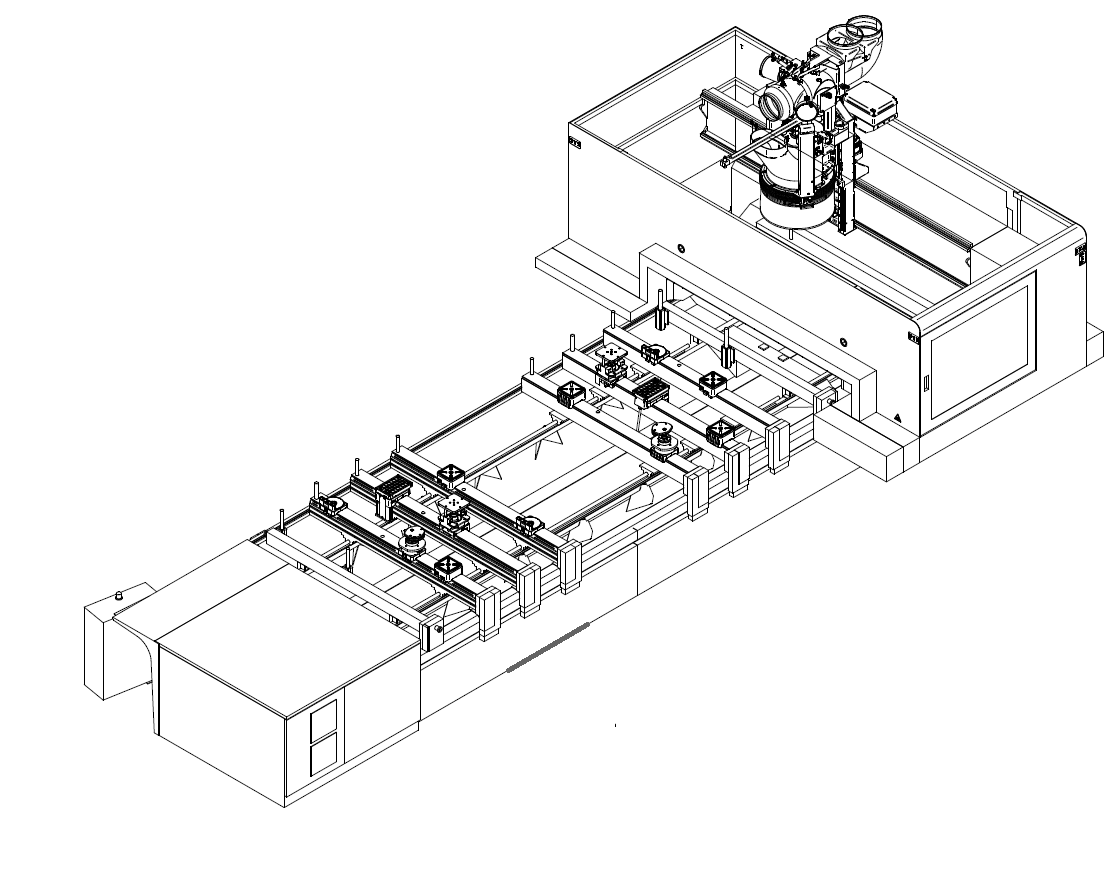
\includegraphics[width=\textwidth]{img/worktable.png}
		\caption{Work center}
		\label{fig:worktable}
	\end{subfigure}
	\hspace{2cm}
	\begin{subfigure}[b]{0.3\textwidth}
		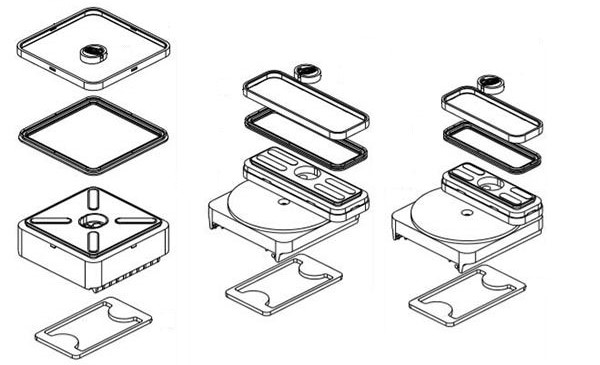
\includegraphics[width=\textwidth]{img/suction_cups_schema_no_dimnesion.jpg}
		\caption{Vacuum suction cup fixtures}
		\label{fig:suction_cups}
	\end{subfigure}
	\caption{On the left, a work center featuring a worktable with movable bars. On the right, fixtures used to secure the workpiece during machining operations.}
	\label{fig:problem_description_img}
\end{figure}


Determining an appropriate fixture layout for a given workpiece is not always straightforward for a human operator, especially when the workpiece has contoured shapes or includes areas to be extruded. Layouts are often based on the operator’s experience; however, such manually designed solutions are not necessarily optimal and can often be improved by considering the structural properties of the fixtures system, such as its resistance to bending and torsional forces.

In this paper, we aim to determine a sound and possibly optimal placement of fixtures beneath the workpiece by identifying, the type, position, and rotation angle of the fixtures that can be used to sustain it. Our approach consists of two stages. First, we compute a feasible, but generally sub-optimal, placement by solving a simplified version of the original problem in which fixture rotations are neglected. To this end, we compare the quality of the solutions obtained using a Constraint Programming (CP) solver and a Reinforcement Learning (RL) algorithm. Second, the resulting layouts are refined through a local search procedure based on Particle Swarm Optimization (PSO), which explicitly accounts for fixture rotations.

This work extends~\cite{vitali2026constraint}, which proposed a hybrid approach combining Constraint Programming (CP), Mixed Integer Programming (MIP), and Particle Swarm Optimization (PSO) to solve the fixture layout optimization problem.  We reformulated several constraints of the CP model, improving its performance on the most challenging instances for the considered solvers, and extend the experimental evaluation by introducing additional real-world case studies. Additionally, we propose a Q-learning-based algorithm for solving the simplified version of the problem and compare its performance with those of the CP and MIP models.

Experimental results show that the solutions produced by the CP and MIP models are of higher quality than those obtained using Q-learning and consistently outperform those designed by an expert operator. Starting from any of these initial layouts, PSO further improves the solution by increasing the moments of inertia of the fixture configuration, thereby enhancing workpiece stability.\footnote{This work was carried out in collaboration with a leading company in the woodworking machinery sector. The name of the company is omitted for privacy reasons.}

\emph{Paper structure.} The paper is organized as follows. Section~\ref{sec:related_work} reviews the related work. Section~\ref{sec:backgorund} presents the background context.  Section~\ref{sec:problem_description} describes the problem parameters and constraints. Section~\ref{sec:cp_model} introduces the CP model, while Section~\ref{sec:mip_model} presents the MIP model. Section~\ref{sec:rl_algorithm} introduces the Q-learning based algorithm. Section~\ref{sec:pso_algorithm} describes the PSO-based algorithm. Finally, Section~\ref{sec:result_analysis} discusses the experimental results, and Section~\ref{sec:conclusions} concludes the paper.

\section{Related Work}
\input{paper_parts/related_work.tex}

\section{Background}
\label{sec:backgorund}
In this section, we introduce the concept of principal moments of inertia. In the proposed resolution strategies, the moments of inertia are used to define the objective function of the fixture layout optimization problem.

\subsection{Principal moments of inertia}

To maximize the stability of the workpiece through fixture placement, the \textit{principal moments} of inertia of the fixture layout system can be analyzed.

The moment of inertia is a geometric property that quantifies a structure’s resistance to bending and torsional forces. It is computed from the distribution of mass relative to a given axis and plays a crucial role in determining the stiffness of structural elements under load. Higher moments of inertia indicate greater resistance to deformation, making this quantity a key factor in the design of fixtures that minimize workpiece deflection during machining operations~\cite{kalkan2013deflection,bischoff2011equivalent}.

To compute the principal moments of inertia of a rectangular fixture system~\cite{belluzzi1961scienza,coultas1925theory,hibbeler2006structural}, each fixture can be represented as a polygon $i$ of $m$ vertices $(x_{i,1}, y_{i,1}), \ldots, (x_{i,m}, y_{i,m})$ with area $A_i$, centroid coordinates $(cx_{i}, cy_{i})$ and rotation angle $\alpha_i$. We first compute the \textit{absolute moments} of inertia of each polygon with respect to the global coordinate system:
%%\begin{gather}
\begin{align*}
	J'_{x,i} 
	&= \tfrac{1}{12} \sum_{j=1}^{m} 
	(y_{i,j}^2 + y_{i,j}y_{i,j+1} + y_{i,j+1}^2)(x_{i,j}y_{i,j+1} - x_{i,j+1}y_{i,j}) \\
	%
	J'_{y,i} 
	&= \tfrac{1}{12} \sum_{j=1}^{m} 
	(x_{i,j}^2 + x_{i,j}x_{i,j+1} + x_{i,j+1}^2) (x_{i,j}y_{i,j+1} - x_{i,j+1}y_{i,j}) \\
	%
	J'_{xy,i} 
	&= \tfrac{1}{24} \sum_{j=1}^{m} 
	(x_{i,j}y_{i,j+1} + 2x_{i,j}y_{i,j} + 2x_{i,j+1}y_{i,j+1} + x_{i,j+1}y_{i,j}) (x_{i,j}y_{i,j+1} - x_{i,j+1}y_{i,j}).
\end{align*}
%%\end{gather}

\noindent The moments of inertia referred to the centroid of each polygon are then computed as:
%%\begin{gather}
\begin{align*}
	J''_{x,i}  = J'_{x,i}  - A_i\,cy_{i}^2, \qquad
	J''_{y,i}  = J'_{y,i}  - A_i\,cx_{i}^2, \qquad
	J''_{xy,i} = J'_{xy,i} - A_i\,cx_{i}\,cy_{i}.
\end{align*}
%%\end{gather}

\noindent Since a polygon can be rotated by an angle $\alpha_i$, the corresponding rotated moments are:
%\begin{gather}
\begin{align*}
	J_{x,i} &= J''_{x,i}\cos^2\alpha_i + J''_{y,i}\sin^2\alpha_i - 2J''_{xy,i}\sin\alpha_i\cos\alpha_i,\\
	J_{y,i} &= J''_{x,i}\sin^2\alpha_i + J''_{y,i}\cos^2\alpha_i - 2J''_{xy,i}\sin\alpha_i\cos\alpha_i,\\
	J_{xy,i} &= (J''_{x,i} - J''_{y,i})\sin\alpha_i\cos\alpha_i + J''_{xy,i}(\cos^2\alpha_i - \sin^2\alpha_i).
\end{align*}
%\end{gather}

\noindent The total moments of inertia with respect to the global axes are then computed as:
%\begin{gather}
\begin{align*}
	J_x &= \sum_{i=1}^{n} J_{x,i} + A_i(cy_{i} - g_y)^2, \qquad
	J_y = \sum_{i=1}^{n} J_{y,i} + A_i(cx_{i} - g_x)^2,\\
	J_{xy} &= \sum_{i=1}^{n} J_{xy,i} + A_i(cx_{i} - g_x)(cy_{i} - g_y)
\end{align*}
%\end{gather}
where $g_x$ and $g_y$ denote the coordinates of the overall centroid of the system, computed as:
%\begin{gather}
\begin{align*}
	g_x = \frac{\sum_{i=1}^{n} A_i\, cx_{i}}{A}, \qquad
	g_y = \frac{\sum_{i=1}^{n} A_i\, cy_{i}}{A}
\end{align*}
%\end{gather}
where $A = \sum_{i=1}^{n} A_i$ is the total area.

\noindent The principal moments of inertia of the overall system are obtained by first evaluating:
%\begin{gather}
\begin{align*}
	J'_{xg} = J_x - A\, g_y^2, \qquad
	J'_{yg} = J_y - A\, g_x^2, \qquad
	J'_{xyg} = J_{xy} - A\, g_x\, g_y,
\end{align*}
%\end{gather}
and then computing:
%\begin{gather}
\begin{align*}
	J_\xi &= \tfrac{1}{2}
	\left(
	(J'_{xg} + J'_{yg})
	- \sqrt{(J'_{xg} - J'_{yg})^2 + 4(J'_{xyg})^2}\,
	\right), \\%[4pt]
	J_\eta &= \tfrac{1}{2}
	\left(
	(J'_{xg} + J'_{yg})
	+ \sqrt{(J'_{xg} - J'_{yg})^2 + 4(J'_{xyg})^2}\,
	\right).
\end{align*}
%\end{gather}

\noindent Layouts that provide good stability for the workpiece are those maximizing the sum:

\begin{equation}
	\finer = J_\xi + J_\eta
	\label{eq:finer}
\end{equation}



\section{Problem description}
\label{sec:problem_description}
Given the workpiece geometry and the available fixture types and quantities, the objective is to determine which fixtures should be selected and their placement so as to maximize workpiece stability during machining.

To ensure the feasibility of a placement, the following constraints must be satisfied:
\begin{enumerate}
	\item the number of fixtures placed for each type must not exceed the number available;
	\item fixtures must be placed so as to satisfy the specified minimum horizontal and vertical safety distances;
	\item fixtures must be positioned within the workpiece boundaries and beneath its surface;
	\item fixtures must not overlap each other;
	\item fixtures must not be located beneath areas to be extruded, to prevent damage.
\end{enumerate}

To illustrate the constraints, Figure~\ref{fig:constraints_axample} shows examples of valid and invalid fixture placements. Fixture $F_6$ is invalid because it violates the minimum horizontal safety distance with respect to fixtures $F_3$ and $F_4$, whereas fixture $F_5$ is invalid because it is positioned beneath an area to be extruded.

\begin{figure}[t]
	\centering
	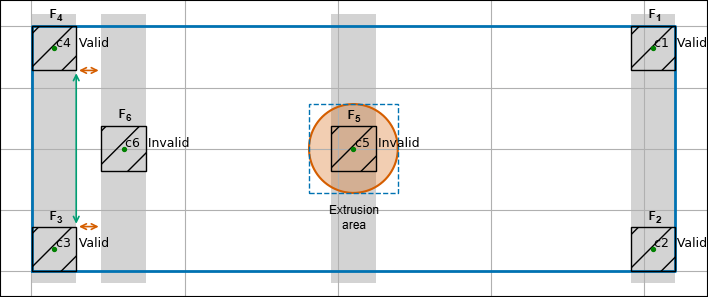
\includegraphics[width=0.65\linewidth]{img/valid_invalid_positions_example.png}
	\caption{Example of valid and invalid fixture placements. For a fixture placement to be valid, the fixture must lie within the workpiece boundaries, satisfy the required safety distances from the other fixtures, and not be positioned beneath an area to be extruded.}
	\label{fig:constraints_axample}
\end{figure}

The formulation of these constraints depends on the chosen solution strategy and the corresponding decision variables and is therefore presented separately for each of the considered solution techniques. All approaches, however, are defined over the same set of input parameters listed below:
\begin{itemize}
	\item the width $\wtab$ and height $\htab$ of the machine worktable;
	\item the minimum horizontal distance $\wmin$ between two fixtures placed on different bars;
	\item the minimum vertical distance $\hmin$ between two fixtures placed on the same bar;
	\item the number $\ntypes$ of different fixture types;
	\item the number $\nfix_i$ of available fixtures for each type $i \in [1..\ntypes]$;
	\item the total number of available fixtures $\nfix = \sum_{i=1}^{\ntypes} \nfix_i$;
	\item the minimum $\nmin$ and maximum $\nmax$ number of fixtures to place;
	\item the width $\wfix_i$ and height $\hfix_i$ of each fixture of type $i$;
	\item the workpiece shape, represented by a set of linear inequalities of the form $\mathtt{a}x + \mathtt{b}y + \mathtt{c} \leq 0$;
	\item the number $\numext$ of areas to be extruded;
	\item the width $\ewside_i$, height $\ehside_i$, and the coordinates $(\xext_i,\yext_i)$ of the lower-left corner of the smallest axis-aligned rectangle enclosing each extrusion area $i \in [1..\numext]$.
\end{itemize}

Extrusion areas are typically represented by simple geometric shapes, such as circles, rectangles, or ellipses, whereas more complex geometries are refined manually. To facilitate the solution process, each extrusion area is approximated by its smallest enclosing rectangle (as illustrated in Figure~\ref{fig:constraints_axample}), which is represented by the coordinates of its lower-left corner together with its width and height.

To evaluate the quality of a fixture layout, two objective functions are considered. The CP and MIP models optimize the objective function $\fdist$ proposed in~\cite{vitali2026constraint}, which maximizes the sum of the pairwise Manhattan distances between fixture centroids, augmented by the total area of the selected fixtures:

\begin{equation}
	\fdist = \sum_{1 \le i < j \le n} \left(|cx_i - cx_j| + |cy_i - cy_j|\right) + \sum_{k=1}^{n} (\wfix_{t_k} \cdot \hfix_{t_k})
	\label{eq:f_dist}
\end{equation}

where $(x_k,y_k)$ are the coordinates of the lower-left corner of the $k$-th placed fixture, having type $t_k$ ($n$ is the total number of placed fixtures), and centroid $(cx_k,cy_k)=\left(x_k+\frac{\wfix_{t_k}}{2},,y_k+\frac{\hfix_{t_k}}{2}\right)$.

The use of the $\fdist$ objective function for the CP and MIP models is motivated by the fact that computing the principal moment of inertia expressed in Eq.~\ref{eq:finer} involves nonlinear operations, including squaring, square roots, and transcendental functions (sine and cosine), which substantially increase the computational effort required by CP and MIP solvers~\cite{leyffer2009applications}.

The Q-learning algorithm, on the other hand, is not affected by the nonlinear computations required to evaluate $\finer$ and therefore directly incorporates the moments of inertia into its reward function, as described in Section~\ref{sec:rl_algorithm}.

The CP model, the MIP model, and the Q-learning algorithm are used to generate initial feasible layouts. For each instance, the best layout produced by these methods is then refined using the PSO algorithm described in Section~\ref{sec:pso_algorithm}, which optimizes $\finer$ while introducing the fixture rotation angle as an additional decision variable.

\section{CP model}
\label{sec:cp_model}

The CP model extends the formulation presented in~\cite{vitali2026constraint} through a revised definition of the decision variables and a reformulation of some constraints, resulting in improved resolution times on the tested instances. The model is defined over the parameters introduced in Section~\ref{sec:problem_description} and maximizes the objective function $\fdist$ defined in Equation~\ref{eq:f_dist}.

\subsection{Variables}
\label{sec:cp_vars}

The fixture placement and type are represented by three arrays of integer decision variables, $x$, $y$, and $t$, for $i = 1,\ldots,\nmax$:
\begin{itemize}
	\item \( (x_i,y_i) \in [0..\wtab]\times [0..\htab] \) denotes the coordinates of the lower-left corner of the $i$-th fixture;
	\item \( t_i \in [0..\ntypes] \) denotes the type of the $i$-th fixture, where type $0$ represents an unused fixture.
\end{itemize}

For each fixture type \(i \in [1..\ntypes]\), an integer variable \(n_i \in [0..\nfix_i]\) denotes the number of selected fixtures of type \(i\), and a variable \(n \in [\nmin..\nmax]\) represents the total number of selected fixtures.

Compared with the formulation presented in~\cite{vitali2026constraint}, the arrays \(x\) and \(y\) and the variable \(n\) are now bounded by \(\nmax\), rather than by \(\nfix\), since the maximum number of fixtures that can be placed is known for each workpiece and $\nmax \leq \nfix$, this tighter bound reduces the search space.

\subsection{Constraints}
\label{sec:cp_cons}

For each fixture type \(i \in [1..\ntypes]\), the \texttt{count} global constraint is used to compute the number of occurrences of value \(i\) in the array \(t\):

\[
n_i = \texttt{count}(t,i).
\]

The total number of selected fixtures is then defined as

\[
n = \sum_{i=1}^{\ntypes} n_i.
\]

Fixture availability is enforced by requiring that the number of selected fixtures of each type does not exceed the number available:

\[
n_i \leq \nfix_i, \qquad \forall i \in [1..\ntypes].
\]

Since not all available fixtures must necessarily be used, we enforce the following invariant:
\[
(i > n) \iff (x_i = \wtab \;\wedge\; y_i = \htab \;\wedge\; t_i = 0), \qquad \forall i \in [1..\nmax].
\]

This invariant ensures that all unused fixtures are assigned the dummy type \(0\) and placed at the dummy location \((\wtab,\htab)\), which lies outside the feasible region.

We guarantee that exactly \(\nmax-n\) fixtures remain unused by imposing

\[
\texttt{count}(t,0) = \nmax - n.
\]


The workpiece shape is defined by linear inequalities of the form \( \mathtt{a}\,x + \mathtt{b}\,y + \mathtt{c} \leq 0 \).
To ensure that each selected fixture \( i \) is placed within the workpiece, we must satisfy
\(
\mathtt{a}\,x'_i + \mathtt{b}\,y'_i + \mathtt{c} \leq 0,
\)
where:
\[
x'_i =
\begin{cases}
	x_i & \text{if } \mathtt{a} \leq 0,\\
	x_i + \wfix_{t_i} & \text{if } \mathtt{a} > 0,
\end{cases}
\qquad
y'_i =
\begin{cases}
	y_i & \text{if } \mathtt{b} \leq 0,\\
	y_i + \hfix_{t_i} & \text{if } \mathtt{b} > 0.
\end{cases}
\]

Areas to be extruded are approximated by axis-aligned rectangles. The non-overlap between these areas and the fixtures is enforced using the \texttt{diffn} global constraint~\cite{DBLP:journals/constraints/BeldiceanuCDP07}. Given a set of rectangles specified by their lower-left corner coordinates and dimensions, the \texttt{diffn} constraint ensures that no two rectangles overlap:
\[
\texttt{diffn}\big(
x \oplus \xext,\;
y \oplus \yext,\;
[\wfix_{t_i} \mid i \in [1..n]] \oplus \ewside,\;
[\hfix_{t_i} \mid i \in [1..n]] \oplus \ehside
\big)
\]
where \( \oplus \) denotes array concatenation. Specifically, we use the non-strict version of \texttt{diffn}, in which zero-width rectangles can be positioned anywhere, ignoring the \( \nmax - n \) unused fixtures.

To enforce the minimum \emph{vertical} distance \( \hmin \) between fixtures placed on the same bar, and the minimum \emph{horizontal} distance \( \wmin \) between fixtures placed on different bars we impose:
\begin{equation*}
	\forall 1 \le i < j \le n: \quad
	\begin{cases}
		y_i + \hfix_{t_i} + \hmin \le y_j
		\;\vee\;
		y_j + \hfix_{t_j} + \hmin \le y_i, & \text{if } cx_i = cx_j,\\[1ex]
		x_i + \wfix_{t_i} + \wmin \le x_j, & \text{if } cx_i \neq cx_j.
	\end{cases}
\end{equation*}
where
\(cx_i\) denotes the $x$-coordinate of the centroid of fixture \( i \).
Centroid coordinates are used instead of lower-left coordinates because fixtures may be wider than their supporting bar: while \( x_i \) may fall outside the horizontal span of the bar, the centroid \( cx_i \) always lies within it.

To compute the fixture centroid coordinates while maintaining integer variables, they are computed using integer division of the fixture dimensions, for each fixture $i \in [1..\nmax]$, we define:

\begin{equation}
	cx_i = x_i + \left\lfloor \frac{\wfix_{t_i}}{2} \right\rfloor, \quad
	cy_i = y_i + \left\lfloor \frac{\hfix_{t_i}}{2} \right\rfloor .
\end{equation}

To improve the propagation of the integer division, the following redundant linear constraints were introduced:

\begin{align*}
	2 \cdot cx_i - 2 \cdot x_i = \wfix_{t_i} - (\wfix_{t_i} \bmod 2), \\
	2 \cdot cy_i - 2 \cdot y_i = \hfix_{t_i} - (\hfix_{t_i} \bmod 2).
\end{align*}

Finally, the model exhibits symmetries whenever fixtures of the same type are permuted without changing their spatial arrangement. To eliminate these equivalent solutions, a lexicographic ordering is imposed on the fixture positions using the \texttt{lex\_chain} global constraint:

\[
(x_{i-1},y_{i-1}) \preceq (x_i,y_i),
\qquad i \in [2..\nmax].
\]

\section{MIP model}
\label{sec:mip_model}

In this section, we present the Mixed-Integer Programming (MIP) formulation for the fixture layout optimization problem. Unlike the CP model, the MIP formulation does not rely on global constraints. Instead, it represents the problem as a system of linear constraints over continuous and binary decision variables. This
relaxation comes from the nature of MIP solving which, unlike most CP solvers, naturally handles
non-negative continuous variables.


\subsection{Variables}
Variables \(x_i\) and \(y_i\), for \(i=1,\dots,\nmax\), have the same semantics as those defined in Section~\ref{sec:cp_vars}, with the only difference that they are continuous rather than discrete.

Fixture types are encoded by a binary matrix \(T\) of size \(\nmax \times \ntypes\), where

\[
T_{i,j} =
\begin{cases}
	1 & \text{if fixture \(i\) is selected and has type \(j\),}\\
	0 & \text{otherwise.}
\end{cases}
\]

To represent the width, height, and type of each fixture, auxiliary variables \(w_i\), \(h_i\), and \(t_i\) are introduced for each \(i \in [1 \ldots \nmax]\).

To linearize the constraints presented in Section~\ref{sec:cp_cons}, the following auxiliary binary variables are defined:

\begin{itemize}
	\item \(\used_i\), which indicates whether fixture \(i\) is selected;
	\item \(\samebar_{i,j}\), which indicates whether fixtures \(i\) and \(j\) are placed on the same bar;
	\item \(\aboveinbar_{i,j}\) and \(\belowinbar_{i,j}\), which indicate whether fixture \(i\) is positioned above or below fixture \(j\) on the same bar;
	\item \(\nooverlapabove_{i,j}\), \(\nooverlapbelow_{i,j}\), \(\nooverlapleft_{i,j}\), and \(\nooverlapright_{i,j}\), which indicate whether fixture \(i\) is positioned above, below, to the left, or to the right of fixture \(j\), respectively;
	\item \(\aboveext_{i,j}\), \(\belowext_{i,j}\), \(\leftext_{i,j}\), and \(\rightext_{i,j}\), which indicate whether fixture \(i\) is positioned above, below, to the left, or to the right of extrusion area \(j\), respectively.
\end{itemize}


\subsection{Constraints}
For each fixture \(i \in [1..\nmax]\), the following equations are imposed:

\[
\used_i = \sum_{j=1}^{\ntypes} T_{i,j}, \qquad
w_i = \sum_{j=1}^{\ntypes} \wfix_j \cdot T_{i,j}, \qquad
h_i = \sum_{j=1}^{\ntypes} \hfix_j \cdot T_{i,j}, \qquad
t_i = \sum_{j=1}^{\ntypes} j \cdot T_{i,j}.
\]

These equations ensure that the width, height, and type assigned to each fixture are consistent and that unused fixtures have dimensions and type equal to \(0\).

To respect fixtures availability constraints, we impose:
\[
\sum_{i=1}^{\nmax} T_{i,j} \le \nfix_j, \quad \forall j \in [1..\ntypes] \qquad\qquad
\nmin \le \sum_{i=1}^{\nmax} \used_i \le \nmax
\]

To determine whether two fixtures lie on the same bar for all \(i \in [1..\nmax]\) and \(j \in [i+1..\nmax]\) we impose the following constraints:
\[
\begin{aligned}
	&\samebar_{i,j} \le \used_i \qquad \samebar_{i,j} \le \used_j \\
	&\samebar_{i,j} = \aboveinbar_{i,j} + \belowinbar_{i,j}\\
	&cx_i - cx_j \le M (1 - \samebar_{i,j}) \qquad cx_j - cx_i \le M (1 - \samebar_{i,j}) \\
\end{aligned}
\]

where \(M = \wtab \cdot \htab\) is the \emph{``big-M''} constant. Then to enforce the appropriate safety distances we use the following inequalities:
\[
\begin{aligned}
	&cx_i + \wmin \le cx_j + M(\samebar_{i,j} + \nooverlapright_{i,j}) \\
	&cx_j + \wmin \le cx_i + M(\samebar_{i,j} + \nooverlapleft_{i,j}) \\
	&y_i + h_i + \hmin - y_j \le M (1 - \aboveinbar_{i,j}) \\
	&y_j + h_j + \hmin - y_i \le M (1 - \belowinbar_{i,j}).
\end{aligned}
\]

To prevent overlap between fixtures, for all \(i,j \in [1..\nmax]\) with \(i < j\), we impose:
\[
\begin{aligned}
	&\nooverlapabove_{i,j} + \nooverlapbelow_{i,j} +
	\nooverlapleft_{i,j} + \nooverlapright_{i,j} \ge 1 \\
	&x_i + w_i \le x_j + M (1 - \nooverlapleft_{i,j}) \qquad
	&y_i + h_i \le y_j + M (1 - \nooverlapbelow_{i,j}) \\
	&x_j + w_j \le x_i + M (1 - \nooverlapright_{i,j}) \qquad
	&y_j + h_j \le y_i + M (1 - \nooverlapabove_{i,j})
\end{aligned}
\]
Analogous constraints are introduced to prevent overlap between fixtures and extrusion areas. For each fixture \(i \in [1..\nmax]\) and extrusion area \(j \in [1..\numext]\), the same inequalities are applied using the binary variables \(\aboveext_{i,j}\), \(\belowext_{i,j}\), \(\leftext_{i,j}\), and \(\rightext_{i,j}\).

The workpiece is defined by linear inequalities of the form $\mathtt{a}x + \mathtt{b}y + \mathtt{c} \leq 0$, so for each fixture \(i \in [1..\nmax]\) we impose \(\mathtt{a}\,x'_i + \mathtt{b}\,y'_i + \mathtt{c} \leq 0\), where \(x'_i\) and \(y'_i\) are defined as in the CP model (see Section~\ref{sec:cp_cons}).

To break symmetries, we enforce an ordering on fixture types: $t_i \ge t_{i+1}$ for $i \in [1..\nmax-1]$.

Finally, the absolute value terms appearing in \(\fdist\) are linearized using a big-\(M\) formulation, unfolding each term of the form \(u=|v|\) into: 

$$u \ge v ~\wedge~ u \ge -v ~\wedge~ u \leq v + M (1 - b)  ~\wedge~ u \leq -v + M b~\wedge~ b\in\{0,1\}.$$

\section{Q-learning algorithm}
\label{sec:rl_algorithm}

We compared the solutions obtained using the CP and MIP models with those produced by a Q-learning based algorithm.

In Q-learning, an agent learns through repeated interactions with the environment by estimating the action-value function \(Q(s,a)\), which represents the expected \textit{cumulative discounted reward}• obtained by executing action \(a\) in state \(s\) and subsequently following the optimal policy~\cite{watkins1992q}.

After each interaction, the action-value function is updated according to the following rule~\cite{krose1995learning}:

\begin{equation}
	Q(s_t,a_t) \leftarrow Q(s_t,a_t)
	+ \alpha
	\left[
	r_{t+1}
	+ \gamma \max_{a_{t+1}}Q(s_{t+1},a_{t+1})
	- Q(s_t,a_t)
	\right],
	\label{eq:update_q}
\end{equation}

where \(\alpha\) is the learning rate, which determines the influence of newly acquired information on the current estimate, and \(\gamma\) is the discount factor, which balances the importance of immediate and future rewards. In Equation~\eqref{eq:update_q}, the quantity inside the square brackets is the \emph{temporal-difference (TD) error}, which measures the difference between the current estimate and the updated estimate obtained after observing the transition from state \(s_t\) to state \(s_{t+1}\). The term \(r_{t+1}\) denotes the reward obtained after executing action \(a_t\), while \(\max_{a_{t+1}}Q(s_{t+1},a_{t+1})\) represents the estimated value of the best action available in the successor state.

In our formulation, the environment corresponds to the considered workpiece. At each decision step, the state of the environment is defined as

\[
s_t=(n_t,fix_t),
\]

where \(n_t\) is the number of fixtures already placed at step \(t\), while
\(fix_t=[fix_t^{1},\,fix_t^{2},\,\ldots,\,fix_t^{\ntypes}]\)
is an integer array of size \(\ntypes\), whose components denote the remaining availability of the different fixture types.

An action consists of selecting a fixture type together with a feasible centroid position,

\[
a_t=(type_t,(cx_t,cy_t)).
\]

The fixture centroid is used as the reference point for positioning instead of the lower-left corner adopted in the CP and MIP models, since it simplifies both the enforcement of the horizontal and vertical safety-distance constraints, as described in Section~\ref{sec:cp_cons}, and the identification of feasible actions.

The action to be executed is selected according to an \textit{\(\epsilon\)-greedy policy}~\cite{sutton1998reinforcement}. At each decision step, the agent selects the action with the highest estimated \(Q\)-value with probability \(1-\epsilon\), whereas with probability \(\epsilon\) it selects a random action, balancing exploration and exploitation of the environment.

The Q-learning based procedure adopted for fixture layout optimization is described in Algorithm~\ref{alg:qlearning_fixtures}. The algorithm takes as inputs the number of training episodes \(E\), the maximum number of steps per episode \(T\), the learning rate \(\alpha\), the discount factor \(\gamma\), the exploration rate \(\epsilon\), and the exploration decay factor \(\rho\). The output is the best feasible fixture layout \(\mathcal{L}^{*}\) obtained by applying the learned policy.

\begin{algorithm}[t]
	\footnotesize
	\caption{Q-learning for Fixture Layout Optimization}
	\label{alg:qlearning_fixtures}
	\begin{algorithmic}[1]
		
		\Require Number of episodes $E$, maximum number of steps per episode $T$, learning rate $\alpha$, discount factor $\gamma$, exploration rate $\epsilon$, exploration decay factor $\rho$
		\Ensure Best feasible layout $\mathcal{L}^*$
		
		\State Compute all candidate centroid positions
		\label{alg:q_init_start}
		\State Remove centroid positions violating the constraints and set $\mathcal{A}(s_1)$
		\State Initialize $Q(s,a)=0$
		\State $\mathcal{L}^* \gets \emptyset$
		\label{alg:q_init_end}
		
		\For{$ep=1$ to $E$}
		\label{alg:q_iteration_start}
		
		\For{$t=1$ to $T$}
		
		% \State Compute the feasible action set $\mathcal{A}(s_t)$
		
		\If{$\mathcal{A}(s_t)=\emptyset$}
		\State \textbf{break}
		\EndIf
		\label{alg:q_iteration_end}
		
		\If{random number $<\epsilon$} \Comment{exploration}
		\label{alg:q_policy_start}
		\State Select a random feasible action
		$a_t \in \mathcal{A}(s_t)$
		\Else \Comment{exploitation}
		\State Select
		$a_t=\arg\max\limits_{a\in\mathcal{A}(s_t)}Q(s_t,a)$
		\EndIf
		
		\State Perform action $a_t$ by placing the selected fixture
		\label{alg:q_policy_end}
		
		\State Recompute the feasible action set $\mathcal{A}(s_{t+1})$ 
		\label{alg:q_reset_action}
		
		\State Compute reward $r_t$ according to Eq.~\ref{eq:reward}
		\label{alg:q_update_start}
		
		\State Observe successor state $s_{t+1}$
		
		\State $Q(s_t,a_t) \gets Q(s_t,a_t) + \alpha \left[r_{t+1} + \gamma \max_{a_{t+1}}Q(s_{t+1},a_{t+1}) - Q(s_t,a_t) \right]$
		
		\State $s_t \gets s_{t+1}$
		\State Update $\mathcal{L}_{ep}$ with $a_t$
		\label{alg:q_update_end}
		
		\EndFor
		
		\If{$\mathcal{L}_{ep}$ is better than $\mathcal{L}^*$}
		\State $\mathcal{L}^* \gets \mathcal{L}_{ep}$
		\EndIf
		\State $\epsilon \gets \rho\,\epsilon$
		\State Reset the environment to the initial state $s_1$
		\State Reset the action space to $\mathcal{A}(s_1)$
		
		\EndFor
		
		\State Evaluate the learned policy using greedy action selection
		\label{alg:q_evaluate_start}
		\State \textbf{return} $\mathcal{L}^*$
		\label{alg:q_evaluate_end}
		
	\end{algorithmic}
\end{algorithm}

Given the fixture dimensions, it is known \emph{a priori} that some positions within the workpiece cannot accommodate a fixture, particularly those near the workpiece boundary or close to areas to be extruded. During the initialization phase, in lines~\ref{alg:q_init_start}--\ref{alg:q_init_end} of Algorithm~\ref{alg:qlearning_fixtures}, centroid positions that would result in fixtures extending outside the workpiece boundaries or overlapping extrusion areas are removed from the set of possible actions \(\mathcal{A}(s_t)\), considering the dimensions of the smallest fixture as reference.

Figure~\ref{fig:q_learning_actions} shows an example of the set of feasible actions for a given workpiece, considering two available fixture types: square and rectangular. Green dots indicate centroid positions where both fixture types can be placed, whereas red dots indicate positions where only rectangular fixtures can be placed.

The algorithm iterates over the training episodes and the corresponding steps. An episode terminates when no feasible actions remain or the maximum number of steps is reached, as shown in lines~\ref{alg:q_iteration_start}--\ref{alg:q_iteration_end} of Algorithm~\ref{alg:qlearning_fixtures}.

The agent selects actions according to the \(\epsilon\)-greedy policy (lines~\ref{alg:q_policy_start}--\ref{alg:q_policy_end} of Algorithm~\ref{alg:qlearning_fixtures}), balancing the exploration of new placements with the exploitation of previously learned actions.

Each action selected is evaluated through the reward associated with the transition from \(s_t\) to \(s_{t+1}\). The reward function combines the improvement obtained in the moment of inertia with additional terms promoting layouts composed of a larger number of fixtures, larger fixture dimensions, and increased spatial separation between fixtures:

\begin{equation}
	r_{t+1}
	=
	\lambda_{\mathrm{iner}}\,\Delta\finer
	+
	\lambda_n n_{t+1}^{2}
	+
	\lambda_d\bar d
	+
	\begin{cases}
		b_{\nmin}, & \text{if } n_{t+1}\geq\nmin,\\
		0, & \text{otherwise}.
	\end{cases}
	\label{eq:reward}
\end{equation}

In the equation: 
\begin{itemize} 
	\item $\Delta\finer$ is the variation of $\finer$ between the previous and current states;
	\item \(n_{t+1}\) is the number of fixtures in the resulting layout. The quadratic term promotes layouts with a larger number of fixtures;
	\item \(\bar d\) is the average Euclidean distance between the newly placed fixture and the previously placed fixtures,  promoting layouts with a larger spatial separation;
	\item \(\lambda_{\finer}\), \(\lambda_n\), and \(\lambda_d\) are weighting coefficients balancing the contribution of the different reward components;
	\item \(b_{\nmin}\) is an additional feasibility bonus assigned when the minimum required number of fixtures, \(\nmin\), has been placed.
\end{itemize}

After each fixture placement, all candidate centroid positions that no longer satisfy the safety-distance constraints are removed from the feasible action set, as shown in line~\ref{alg:q_reset_action} of Algorithm~\ref{alg:qlearning_fixtures}. Consequently, the action set progressively shrinks as the layout is constructed, ensuring that all geometric constraints are satisfied.

The only constraint that cannot be enforced by restricting the feasible action set is the placement of the minimum number of required fixtures \(\nmin\). For this reason, the feasibility bonus \(b_{\nmin}\) is included in the reward function to encourage the agent to generate layouts satisfying this constraint.

After executing the selected action, the corresponding reward is computed, the \(Q\)-function value associated with state \(s_t\) and action \(a_t\) is evaluated and the learned policy is updated (lines~\ref{alg:q_update_start}--\ref{alg:q_update_end} of Algorithm~\ref{alg:qlearning_fixtures}).

Finally, after all training episodes have been completed, the learned policy is evaluated to obtain the fixture layout for the considered workpiece, as shown in lines~\ref{alg:q_evaluate_start}--\ref{alg:q_evaluate_end} of Algorithm~\ref{alg:qlearning_fixtures}.

\begin{figure}[t]
	\centering
	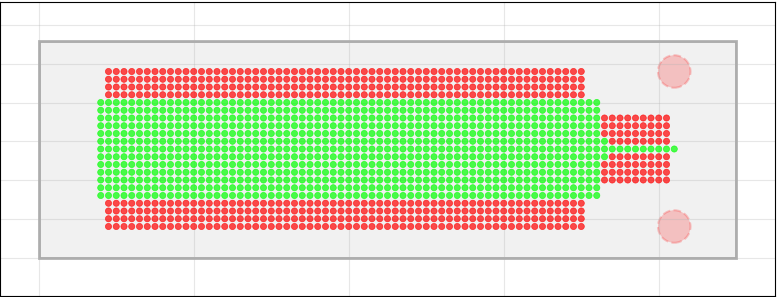
\includegraphics[width=0.5\linewidth]{img/q_learning_actions.png}
	\caption{Example of the available actions for a given workpiece. Green dots represent centroid positions where both square and rectangular fixtures can be placed, whereas red dots represent positions where only rectangular fixtures can be placed. The workpiece area is highlighted in light gray, while the areas to be extruded are highlighted in red.}
	\label{fig:q_learning_actions}
\end{figure}


\section{PSO algorithm}
\label{sec:pso_algorithm}

Particle Swarm Optimization (PSO) is employed as a meta-heuristic refinement procedure, using the solutions obtained from the CP model, the MIP models and the Q-learning-based approach, as starting layouts. 

PSO is an iterative optimization technique inspired by swarm intelligence and originally motivated by studies of the collective behavior of bird flocks~\cite{sun2022particle,liu2006solving}. The meta-heuristic operates on a swarm of particles, each characterized by a position vector \(p_i\) and a velocity vector \(v_i\). The position of each particle represents a candidate solution and is associated with a fitness value measuring its quality. At each iteration \(t=1,2,\ldots\), particles explore the search space by updating their velocities and positions according to the following equations:

\begin{align*}
	v_i^{(t+1)} &= w \, v_i^{(t)}
	+ c_1 r_1 \big( p_i^* - p_i^{(t)} \big)
	+ c_2 r_2 \big( g^* - p_i^{(t)} \big) \\
	p_i^{(t+1)} &= p_i^{(t)} + v_i^{(t+1)}
\end{align*}

where:
\begin{itemize}
	\item \(w\) is the \emph{inertia weight}, controlling how much of the previous velocity is retained;
	\item \(c_1\) is the \emph{cognitive coefficient}, guiding the particle toward its \emph{personal best position} \(p_i^*\);
	\item \(c_2\) is the \emph{social coefficient}, guiding particles toward the \emph{global best position} \(g^*\) of the swarm;
	\item \(r_1\) and \(r_2\) are random numbers uniformly distributed in \([0,1]\), introducing stochasticity into the cognitive and social components, respectively.
\end{itemize}

In the proposed approach, PSO further improves the provided initial layouts by explicitly considering fixture rotation. The objective is to maximize the sum of the principal moments of inertia, i.e., the objective function \(\finer = J_\xi + J_\eta\) defined in Section~\ref{sec:backgorund}.

In our formulation, the position of each particle \(s \in [1,\swarmsize]\) is represented by a matrix \(P_s\) with four rows and \(\nmax\) columns. Each column of \(P_s\) represents a fixture, while each row corresponds to one of the decision variables:
\begin{itemize}
	\item $P_s[1,j]$: the $x$-coordinate of the lower-left corner of the $j$-th fixture;
	\item $P_s[2,j]$: the $y$-coordinate of the lower-left corner of the $j$-th fixture;
	\item $P_s[3,j]$: the type $t$ associated with the $j$-th fixture;
	\item $P_s[4,j]$: the rotation angle $\alpha$ of the $j$-th fixture.
\end{itemize}

Each position matrix $P_s$ represents a candidate solution associated with particle $s$. The availability of an initial solution obtained from the CP model, the MIP model, or the Q-learning algorithm, ensures that the swarm is initialized from feasible layouts.


\begin{algorithm}[htbp]
	\footnotesize
	\caption{Particle Swarm Optimization for Fixture Layout Optimization}
	\label{alg:pso_fixtures}
	\begin{algorithmic}[1]
		\Require Swarm size $\swarmsize$, maximum number of iterations $\maxiter$, inertia weight $w$, cognitive coefficient $c_1$,
		social coefficient $c_2$, variable bounds, initial solution $P_0$, maximum number of fixtures $\nmax$
		\Ensure Feasible solution $P^*$ not worse than $P_0$
		
		\For{$s = 1$ to $\swarmsize$}
		\label{alg:start_init}
		\If{$s = 1$}
		\State $P^* \gets P^*_s \gets P_s \gets P_0$
		\Else
		\State $P^*_s \gets P_s \gets P_0 + \text{random perturbation}$
		\EndIf
		\label{alg:end_init}
		
		\If{$cv(P_s)=0$}
		\label{alg:start_init_eval}
		\If{$\finer(P_s)>\finer(P^*)$}
		\State $P^*\gets P_s$
		\EndIf
		\EndIf
		\label{alg:end_init_eval}
		
		\State Randomly initialize velocity matrix $V_s$
		\EndFor
		
		\For{$k=1$ to $\maxiter$}
		\For{$s=1$ to $\swarmsize$}
		\For{$i=1$ to $4$}
		\For{$j=1$ to $\nmax$}
		\Comment{Update velocity and position}
		\State Randomly generate $r_1,r_2\in[0,1]$
		\label{alg:start_pso_update}
		\State $V_s[i,j]\gets wV_s[i,j]+c_1r_1(P^*_s[i,j]-P_s[i,j])+c_2r_2(P^*[i,j]-P_s[i,j])$
		\State $P_s[i,j]\gets P_s[i,j]+V_s[i,j]$
		\label{alg:end_pso_update}
		\EndFor
		\EndFor
		
		\For{$j=1$ to $\nmax$}
		\If{fixture $j$ lies outside the workpiece}
		\label{alg:start_fixing_geom}
		\State Identify the nearest workpiece vertex and the fixture vertex farthest from it
		\State Translate fixture $j$ by the minimum displacement required to satisfy the boundary constraint
		\label{alg:end_fixing_geom}
		\EndIf
		
		\If{fixture $j$ has type 0}
		\label{alg:start_fixing_type}
		\State Set $P_s[1,j]\gets\wtab$ and $P_s[2,j]\gets\htab$
		\EndIf
		\label{alg:end_fixing_type}
		\EndFor
	
		
		\If{$cv(P_s)=0$ \textbf{and} $cv(P^*_s)=0$}
		\Comment{Deb's rules}
		\label{alg:start_deb_eval}
		\If{$\finer(P_s)>\finer(P^*_s)$}
		\State $P^*_s\gets P_s$
		\If{$\finer(P^*_s)>\finer(P^*)$}
		\State $P^*\gets P^*_s$
		\EndIf
		\EndIf
		\ElsIf{$cv(P_s)<cv(P^*_s)$}
		\State $P^*_s\gets P_s$
		\EndIf
		\label{alg:end_deb_eval}
		
		\EndFor
		\EndFor
		
		\State \Return $P^*$
		
	\end{algorithmic}
\end{algorithm}


Algorithm~\ref{alg:pso_fixtures} presents the pseudocode of the implemented PSO approach. Given the swarm size \(\swarmsize\), the maximum number of iterations \(\maxiter\), the inertia weight \(w\), the cognitive coefficient \(c_1\), the social coefficient \(c_2\), the variable bounds, the initial feasible layout \(P_0\), and the maximum number of fixtures \(\nmax\), the algorithm returns the optimized feasible fixture layout \(P^*\).

During the initialization phase (lines~\ref{alg:start_init}--\ref{alg:end_init} of Algorithm~\ref{alg:pso_fixtures}), the first particle is assigned the provided initial solution $P_0$, whereas the remaining particles are initialized using randomly perturbed versions of $P_0$. The velocity matrix $V_s$ of each particle $s$, which stores the velocity components corresponding to each element of the position matrix $P_s$, is randomly initialized, and the personal best position $P^*_s$ is initially set equal to the particle’s starting position.

In this formulation, the linear constraints of the MIP model are incorporated into the PSO framework and treated as soft constraints, with the non-overlap constraints adapted to account for fixture rotations. Accordingly, for each particle position $P_s$, the violation of the $j$-th constraint is evaluated by means of a binary function $cv_j(P_s)$, which indicates whether the constraint is violated or satisfied. The overall constraint violation $cv(P_s)$ for position $P_s$ is computed as the sum of each individual constraint violation.

Once all particles have been initialized, they are evaluated in terms of the objective function $\finer(P_s)$ and the constraint violation $cv(P_s)$, as reported in lines~\ref{alg:start_init_eval}--\ref{alg:end_init_eval} of Algorithm~\ref{alg:pso_fixtures}. Based on this evaluation, the global best position of the swarm, denoted by $P^*$, is identified.

When fixtures are axis-aligned, non-overlap can be enforced through coordinate-wise comparisons by exploiting the orientation of the rectangle edges. Introducing fixture rotations invalidates this criterion, since the global position of each vertex depends on the rotation angle and must be computed through trigonometric transformations. Consequently, non-overlap verification becomes orientation-dependent, increasing the implementation complexity. Furthermore, vertex-based checks are no longer sufficient for oriented rectangles, as two fixtures may intersect even when no vertex of either rectangle lies inside the other, for example in edge-to-edge configurations.

For this reason, the \emph{Separation Axis Theorem} (SAT)~\cite{liang2015research} is adopted to enforce the non-overlap constraint. The theorem states that two oriented rectangles do not overlap if and only if there exists at least one axis along which their projections are disjoint. Such an axis is called a \emph{separating axis}. Therefore, non-overlap is verified by projecting both rectangles onto the candidate separating axes and checking whether their projections are disjoint on at least one of them, as illustrated in Figure~\ref{fig:sat_theorem}.

\begin{figure}[t]
	\centering
	\begin{subfigure}{0.45\textwidth}
		\centering
		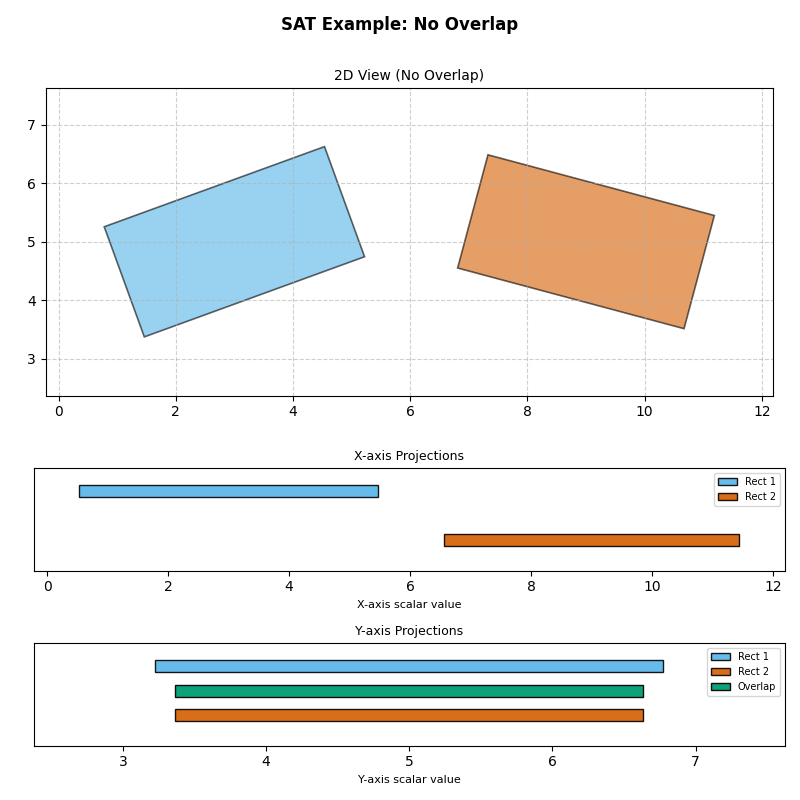
\includegraphics[width=\textwidth]{img/sat_no_overlap_colored.png}
		\caption{Separation Axis Theorem with no overlap}
		\label{fig:1a_sat}
	\end{subfigure}
	\hfill
	\begin{subfigure}{0.45\textwidth}
		\centering
		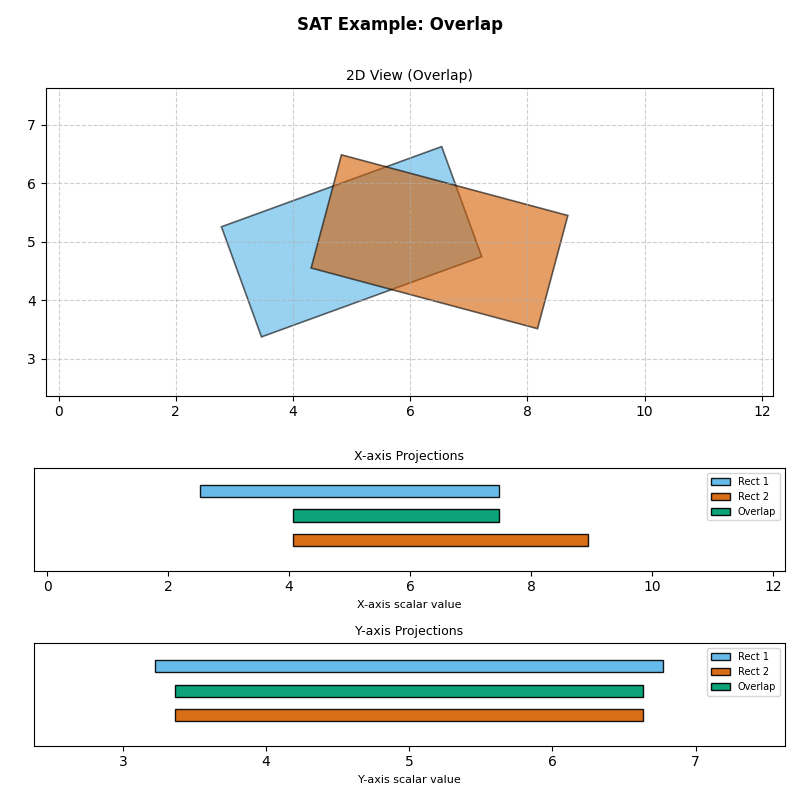
\includegraphics[width=\textwidth]{img/sat_overlap_colored.png}
		\caption{Separation Axis Theorem with overlap}
		\label{fig:1b_sat}
	\end{subfigure}
	
	\caption{Separation Axis Theorem for oriented rectangles. Each figure consists of three subplots. The first subplot illustrates the spatial configuration of the rectangles. The second and third subplots show the projections of their principal axes onto the $x$- and $y$-axes, respectively. An overlap occurs when the projections intersect along both axes; the overlap is highlighted in black in the second and third subplots.}
	\label{fig:sat_theorem}
\end{figure}

During the search phase (lines~\ref{alg:start_pso_update}--\ref{alg:end_pso_update} of Algorithm~\ref{alg:pso_fixtures}), the velocity matrix $V_s$ and the position matrix $P_s$ associated with particle $s$ are iteratively updated according to the standard PSO update equations.

Whenever possible, constraint violations arising from updated fixture positions are mitigated through dedicated geometric repair procedures, as reported in lines~\ref{alg:start_fixing_geom}--\ref{alg:end_fixing_geom} of Algorithm~\ref{alg:pso_fixtures}. For each fixture, if its geometry lies partially or entirely outside the workpiece boundary, the nearest vertex of the workpiece polygon and the fixture vertex farthest from it are identified. The fixture is then translated by the minimum displacement required to satisfy the boundary constraint. The repair strategy is limited to geometric violations, as these constraints are the most suitable for correction without adversely affecting the satisfaction of other constraints.

In lines~\ref{alg:start_fixing_type}--\ref{alg:end_fixing_type} of Algorithm~\ref{alg:pso_fixtures}  fixtures with type zero, representing unused fixtures, are assigned the dummy lower-left corner coordinates \((\wtab,\htab)\), as in the CP model formulation (see Section~\ref{sec:cp_cons}), and are excluded from constraint violation evaluations.

To guide the search toward constraint-respecting positions, as illustrated in lines~\ref{alg:start_deb_eval}--\ref{alg:end_deb_eval} of Algorithm~\ref{alg:pso_fixtures}, candidate solutions are evaluated using Deb’s rules~\cite{deb2000efficient}:
\begin{itemize}
	\item Between two feasible solutions, retain the one with the higher objective value.
	\item Between a feasible and an infeasible solution, retain the feasible one.
	\item Between two infeasible solutions, retain the one with the lower constraint violation.
\end{itemize}

After updating the personal best position $P^*_s$ of each particle $s$ using Deb’s rules, the global best position $P^*$ of the swarm is updated accordingly. At the end of the final iteration, the best position found by the swarm is returned.

\section{Evaluation}
\label{sec:result_analysis}

We evaluated the proposed resolution strategy on seven distinct workpieces: a stair step of a spiral staircase, a stair step of a simple staircase, a music speaker, a dashboard, a coffee table, a door, and a door with a porthole (see Table~\ref{tab:visual_results}).

The work center considered was equipped with 24 square fixtures with dimensions \(145 \times 145\)~mm and 12 rectangular fixtures with dimensions \(180 \times 65\)~mm. The minimum and maximum numbers of fixtures were set to \(\nmin = 3\) and \(\nmax = 6\), respectively, for all workpieces except the coffee table and the two door workpieces, which, due to their larger dimensions, required \(\nmin = 6\) and \(\nmax = 10\), and \(\nmin = 10\) and \(\nmax = 20\), respectively.

Both the CP and MIP models were implemented in \textit{MiniZinc} version~2.9.5~\cite{nethercote2007MiniZinc}. The CP model was solved using the CP solvers Gecode~\cite{schulte2006gecode}, Chuffed~\cite{chuffed}, and OR-Tools~\cite{ortools}, whereas the MIP model was solved using the commercial solver Gurobi~\cite{gurobi}.

We also considered \(\lns\), a variant of Gecode implementing Large Neighborhood Search (LNS)~\cite{pisinger2018large}, to solve the CP model, configuring it to explore the search space by randomly fixing 80\% of the decision variables corresponding to the \(x\)- and \(y\)-coordinates, adopting a constant restart strategy triggered every 1000 explored nodes.

All solvers were executed in single-threaded mode to ensure a fair comparison. The experiments were performed on a 64-bit Windows machine equipped with an Intel Core i5 processor and 16~GB of RAM.

\begin{table}[!b]
	\centering
	\footnotesize
	\caption{Objective values for $\fdist$ and $\finer$, and solve time $t_{solve}$ in seconds to reach the best $\fdist$ solution. Timeout (300~s) is indicated by ``--''. Solutions where the solver reached optimality are marked with $^*$. For each workpiece, the maximum values of $\fdist$ and $\finer$ are highlighted in bold, including ties.}
	\label{tab:objective_runtime}
	\setlength{\tabcolsep}{2pt}
	\begin{tabular}{llccccc}
		\toprule
		Workpiece & Metric & Gecode & \lns & Chuffed & OR-Tools & Gurobi \\
		\midrule
		
		\multirow{3}{*}{\makecell{Stair step\\spiral staircase}} & $\fdist$ & $45655{}^*$ & $45655$ & $45655{}^*$ & $45655{}^*$ & $\mathbf{45662.155{}^*}$ \\
		& $\finer$ & \cellcolor{gray!15}$2.13968\times 10^{9}$ & \cellcolor{gray!15}$2.13968\times 10^{9}$ & \cellcolor{gray!15}$2.13960\times 10^{9}$ & \cellcolor{gray!15}$2.13968\times 10^{9}$ & \cellcolor{gray!15}$\mathbf{2.17089\times 10^{9}}$ \\
		& $t_{solve}$ & 0.559 & -- & 0.326 & 0.120 & 2.930 \\
		\midrule
		
		\multirow{3}{*}{\makecell{Stair step\\simple staircase}} & $\fdist$ & $72823$ & $72823$ & $72823{}^*$ & $72721$ & $\mathbf{72826.000{}^*}$ \\
		& $\finer$ & \cellcolor{gray!15}$6.76573\times 10^{9}$ & \cellcolor{gray!15}$6.76573\times 10^{9}$ & \cellcolor{gray!15}$6.76530\times 10^{9}$ & \cellcolor{gray!15}$6.48172\times 10^{9}$ & \cellcolor{gray!15}$\mathbf{6.76638\times 10^{9}}$ \\
		& $t_{solve}$ & -- & -- & 3.386 & -- & 0.220 \\
		\midrule
		
		\multirow{3}{*}{\makecell{Dashboard}} & $\fdist$ & $\mathbf{55582{}^*}$ & $\mathbf{55582}$ & $\mathbf{55582{}^*}$ & $\mathbf{55582{}^*}$ & $\mathbf{55582.000{}^*}$ \\
		& $\finer$ & \cellcolor{gray!15}$\mathbf{7.10094\times 10^{9}}$ & \cellcolor{gray!15}$\mathbf{7.10094\times 10^{9}}$ & \cellcolor{gray!15}$7.08735\times 10^{9}$ & \cellcolor{gray!15}$7.08735\times 10^{9}$ & \cellcolor{gray!15}$7.08735\times 10^{9}$ \\
		& $t_{solve}$ & 0.044 & -- & 0.057 & 0.102 & 0.157 \\
		\midrule
		
		\multirow{3}{*}{\makecell{Speaker}} & $\fdist$ & $\mathbf{49548{}^*}$ & $\mathbf{49548}$ & $\mathbf{49548{}^*}$ & $\mathbf{49548{}^*}$ & $\mathbf{49548.000{}^*}$ \\
		& $\finer$ & \cellcolor{gray!15}$\mathbf{2.93433\times 10^{9}}$ & \cellcolor{gray!15}$\mathbf{2.93433\times 10^{9}}$ & \cellcolor{gray!15}$\mathbf{2.93433\times 10^{9}}$ & \cellcolor{gray!15}$\mathbf{2.93433\times 10^{9}}$ & \cellcolor{gray!15}$\mathbf{2.93433\times 10^{9}}$ \\
		& $t_{solve}$ & 165.018 & -- & 0.106 & 0.120 & 0.126 \\
		\midrule
		
		\multirow{3}{*}{\makecell{Coffee table}} & $\fdist$ & $137262$ & $185351$ & $192711$ & $122920$ & $\mathbf{201686.505}$ \\
		& $\finer$ & \cellcolor{gray!15}$2.20750\times 10^{10}$ & \cellcolor{gray!15}$2.19967\times 10^{10}$ & \cellcolor{gray!15}$\mathbf{2.21449\times 10^{10}}$ & \cellcolor{gray!15}$9.10490\times 10^{9}$ & \cellcolor{gray!15}$2.19472\times 10^{10}$ \\
		& $t_{solve}$ & -- & -- & -- & -- & -- \\
		\midrule
		
		\multirow{3}{*}{\makecell{Door}} & $\fdist$ & $261757$ & $\mathbf{521632}$ & -- & -- & $355744.000$ \\
		& $\finer$ & \cellcolor{gray!15}$1.08442\times 10^{11}$ & \cellcolor{gray!15}$\mathbf{1.52925\times 10^{11}}$ & \cellcolor{gray!15}-- & \cellcolor{gray!15}-- & \cellcolor{gray!15}$1.17690\times 10^{11}$ \\
		& $t_{solve}$ & -- & -- & -- & -- & -- \\
		\midrule
		
		\multirow{3}{*}{\makecell{Door\\with porthole}} & $\fdist$ & $261759$ & $\mathbf{393343}$ & -- & -- & $298186.000$ \\
		& $\finer$ & \cellcolor{gray!15}$1.08422\times 10^{11}$ & \cellcolor{gray!15}$\mathbf{1.52861\times 10^{11}}$ & \cellcolor{gray!15}-- & \cellcolor{gray!15}-- & \cellcolor{gray!15}$1.39714\times 10^{11}$ \\
		& $t_{solve}$ & -- & -- & -- & -- & -- \\
		
		\bottomrule
	\end{tabular}
\end{table}


%\begin{table}[t]
%	\centering
%	\footnotesize
%	\caption{Objective values for $\fdist$ and $\finer$. Solutions where the solver reached optimality (runtime $< 300$ s) are marked with $^*$. For each workpiece, the maximum values of $\fdist$ and $\finer$ are highlighted in bold, including ties. Note that solutions equivalent in terms of $\fdist$ may differ in $\finer$, hence different entries may be highlighted.}
%	\label{tab:objective}
%	\setlength{\tabcolsep}{2pt}
%	\begin{tabular}{llccccc}
%		\toprule
%		Workpiece & Obj. & Gecode & \lns & Chuffed & OR-Tools & Gurobi \\
%		\midrule
%		
%		\multirow{2}{*}{\makecell{Stair step\\spiral staircase}} & $\fdist$ & 45655$^*$ & 45655 & 45655$^*$ & 45655$^*$ & \textbf{45662.155}$^*$ \\
%		& $\finer$ & \cellcolor{gray!15}$2.13968\times 10^{9}$ & \cellcolor{gray!15}$2.13968\times 10^{9}$ & \cellcolor{gray!15}$2.13960\times 10^{9}$ & \cellcolor{gray!15}$2.13968\times 10^{9}$ & \cellcolor{gray!15}$\mathbf{2.17089\times 10^{9}}$ \\
%		\midrule
%		
%		\multirow{2}{*}{\makecell{Stair step\\simple staircase}} & $\fdist$ & 72823 & 72823 & 72823$^*$ & 72721 & \textbf{72826}$^*$ \\
%		& $\finer$ & \cellcolor{gray!15}$6.76573\times 10^{9}$ & \cellcolor{gray!15}$6.76573\times 10^{9}$ & \cellcolor{gray!15}$6.76530\times 10^{9}$ & \cellcolor{gray!15}$6.48172\times 10^{9}$ & \cellcolor{gray!15}$\mathbf{6.76638\times 10^{9}}$ \\
%		\midrule
%		
%		\multirow{2}{*}{\makecell{Dashboard}} & $\fdist$ & \textbf{55582}$^*$ & \textbf{55582} & \textbf{55582}$^*$ & \textbf{55582}$^*$ & \textbf{55582}$^*$ \\
%		& $\finer$ & \cellcolor{gray!15}$\mathbf{7.10094\times 10^{9}}$ & \cellcolor{gray!15}$\mathbf{7.10094\times 10^{9}}$ & \cellcolor{gray!15}$7.08735\times 10^{9}$ & \cellcolor{gray!15}$7.08735\times 10^{9}$ & \cellcolor{gray!15}$7.08735\times 10^{9}$ \\
%		\midrule
%		
%		\multirow{2}{*}{\makecell{Speaker}} & $\fdist$ & \textbf{49548}$^*$ & \textbf{49548} & \textbf{49548}$^*$ & \textbf{49548}$^*$ & \textbf{49548}$^*$\\
%		& $\finer$ & \cellcolor{gray!15}$\mathbf{2.93433\times 10^{9}}$ & \cellcolor{gray!15}$\mathbf{2.93433\times 10^{9}}$ & \cellcolor{gray!15}$\mathbf{2.93433\times 10^{9}}$ & \cellcolor{gray!15}$\mathbf{2.93433\times 10^{9}}$ & \cellcolor{gray!15}$\mathbf{2.93433\times 10^{9}}$ \\
%		\midrule
%		
%		\multirow{2}{*}{\makecell{Coffee table}} & $\fdist$ & 137262 & 185351 & 192711 & 122920 & \textbf{201686.505} \\
%		& $\finer$ & \cellcolor{gray!15}$2.20750\times 10^{10}$ & \cellcolor{gray!15}$2.19967\times 10^{10}$ & \cellcolor{gray!15}$\mathbf{2.21449\times 10^{10}}$ & \cellcolor{gray!15}$9.10490\times 10^{9}$ & \cellcolor{gray!15}$2.19472\times 10^{10}$ \\
%		\midrule
%		
%		\multirow{2}{*}{\makecell{Door}} & $\fdist$ & 261757 & \textbf{521632} & -- & -- & 355744 \\
%		& $\finer$ & \cellcolor{gray!15}$1.08442\times 10^{11}$ & \cellcolor{gray!15}$\mathbf{1.52925\times 10^{11}}$ & \cellcolor{gray!15}-- & \cellcolor{gray!15}-- & \cellcolor{gray!15}$1.17690\times 10^{11}$ \\
%		\midrule
%		
%		\multirow{2}{*}{\makecell{Door\\with porthole}} & $\fdist$ & 261759 & \textbf{393343} & -- & -- & 298186 \\
%		& $\finer$ & \cellcolor{gray!15}$1.08422\times 10^{11}$ & \cellcolor{gray!15}$\mathbf{1.52861\times 10^{11}}$ & \cellcolor{gray!15}-- & \cellcolor{gray!15}-- & \cellcolor{gray!15}$1.39714\times 10^{11}$ \\
%		
%		\bottomrule
%	\end{tabular}
%\end{table}

%\begin{table}[t]
%	\centering
%	\footnotesize
%	\caption{Solve time in seconds to reach the best $\fdist$ solution. Timeout (300~s) is indicated by ``--''.}
%	\label{tab:runtime}
%	%\rowcolors{2}{gray!15}{white}
%	\begin{tabular}{cccccc}
	%		\toprule
	%		Workpiece & Gecode & \lns & Chuffed & OR-Tools & Gurobi \\
	%		\midrule
	%		
	%		\makecell{Stair step\\spiral staircase} & 0.559 & -- & 0.326 & 0.120 & 2.930 \\
	%		\midrule
	%		
	%		\makecell{Stair step\\simple staircase} & -- & -- & 3.386 & -- & 0.220 \\
	%		\midrule
	%		
	%		\makecell{Dashboard} & 0.044 & -- & 0.057 & 0.102 & 0.157 \\
	%		\midrule
	%		
	%		\makecell{Speaker} & 165.018 & -- & 0.106 & 0.120 & 0.126 \\
	%		\midrule
	%		
	%		\makecell{Coffee table} & -- & -- & -- & -- & -- \\
	%		\midrule
	%		
	%		\makecell{Door} & -- & -- & -- & -- & -- \\
	%		\midrule
	%		
	%		\makecell{Door\\with porthole} & -- & -- & -- & -- & -- \\
	%		
	%		\bottomrule
	%	\end{tabular}
%\end{table}

Table~\ref{tab:objective_runtime} reports the values obtained for the objective function $\fdist$ for the different workpieces, together with the corresponding \emph{a posteriori} values of $\finer$, and the solve time $t_{solve}$ required to reach the optimal solution. 

Identical values of $\fdist$ do not necessarily correspond to identical values of $\finer$, as observed for the Dashboard workpiece. This is because the moments of inertia are highly sensitive to little displacement; therefore, if the solutions obtained by the solvers do not result in identical fixture placements, the value of $\finer$ may differ. 

Among the CP solvers, Gecode delivers the best overall performance, finding feasible solutions for all the considered workpieces, whereas Chuffed and OR-Tools fail to find feasible solutions for the two door workpieces.

$\lns$ achieves the best results for the two door workpieces, producing layouts that outperform those obtained by Gurobi with the MIP model. For the remaining workpieces, however, Gurobi finds solutions that are either superior or equivalent to those obtained by the CP solvers with respect to $\fdist$. This can be partly attributed to the use of continuous decision variables in the MIP model, which enlarges the feasible region and may therefore yield higher-quality solutions.

If we consider the information of the solve time presented in Table~\ref{tab:objective_runtime}, among the CP solvers, with an imposed time limit of 300~s, Chuffed is the most robust, finding the optimal solution in four of the seven instances, and it is the only CP solver able to prove optimality for the stiar step of the simple staircase. Gecode exhibits the greatest variability in performance, ranging from competitive runtimes on the easier instances to requiring 165.018~s for the speaker workpiece, while Chuffed and OR-Tools solve the same instance in only 0.106~s and 0.120~s, respectively.

Being a local-search-based approach, $\lns$ cannot prove optimality. Nevertheless, it reaches the same optimal value of $\fdist$ as the other CP solvers for the simpler workpieces and achieves the best value of $\finer$ in four out of the seven considered workpieces, demonstrating the effectiveness of a local search strategy.

The Q-learning-based algorithm was implemented in Python~3.11.9 using the Gymnasium library version~1.3.0. The agent was trained on all the considered workpieces for 200 episodes, each consisting of 20 steps, using the following hyperparameters: learning rate $\alpha = 0.1$, discount factor $\gamma = 0.99$, initial exploration rate $\epsilon = 1.0$, and exploration decay factor $\rho = 0.995$.

Table~\ref{tab:comparison} reports the results obtained for the different workpieces, comparing the corresponding values of the moment of inertia with those achieved by the best CP solver and the MIP model.

Overall, the Q-learning-based algorithm does not outperform either the CP or the MIP model. On average, the values of $\finer$ obtained by RL are 13\% lower than those achieved by CP and 8\% lower than those obtained with MIP. The only exception is the door with a porthole workpiece, for which Q-learning outperforms the solution returned by Gurobi for the MIP model.


\begin{table}[t]
	\centering
	\footnotesize
	\caption{Objective values $\finer$ comparison: CP solvers (best among Gecode, LNS, Chuffed, OR-Tools), MIP solver (Gurobi), and RL approach. For each workpiece, the maximum value is highlighted in bold.}
	\label{tab:comparison}
	\setlength{\tabcolsep}{5pt}
	\begin{tabular}{cccc}
		\toprule
		Workpiece & CP model & MIP model & Q-learning \\
		\midrule
		
		\makecell{Stair step\\spiral staircase} & $2.13968\times 10^{9}$ & $\mathbf{2.17089\times 10^{9}}$ & $1.93822\times 10^{9}$ \\
		\midrule
		
		\makecell{Stair step\\simple staircase} & $6.76573\times 10^{9}$ & $\mathbf{6.76638\times 10^{9}}$ & $5.65433\times 10^{9}$ \\
		\midrule
		
		\makecell{Dashboard} & $\mathbf{7.10094\times 10^{9}}$ & $7.08735\times 10^{9}$ & $6.65446\times 10^{9}$ \\
		\midrule
		
		\makecell{Speaker} & $\mathbf{2.93433\times 10^{9}}$ & $\mathbf{2.93433\times 10^{9}}$ & $2.81248\times 10^{9}$ \\
		\midrule
		
		\makecell{Coffee table} & $\mathbf{2.29750\times 10^{10}}$ & $2.19472\times 10^{10}$ & $1.56444\times 10^{10}$ \\
		\midrule
		
		\makecell{Door} & $\mathbf{1.52925\times 10^{11}}$ & $1.17690\times 10^{11}$ & $1.14387\times 10^{11}$ \\
		\midrule
		
		\makecell{Door\\with porthole} & $\mathbf{1.52861\times 10^{11}}$ & $1.39714\times 10^{11}$ & $1.45467\times 10^{11}$ \\
		
		\bottomrule
	\end{tabular}
\end{table}


\begin{figure}[t]
	\centering
	\begin{subfigure}[b]{\textwidth}
		\centering
		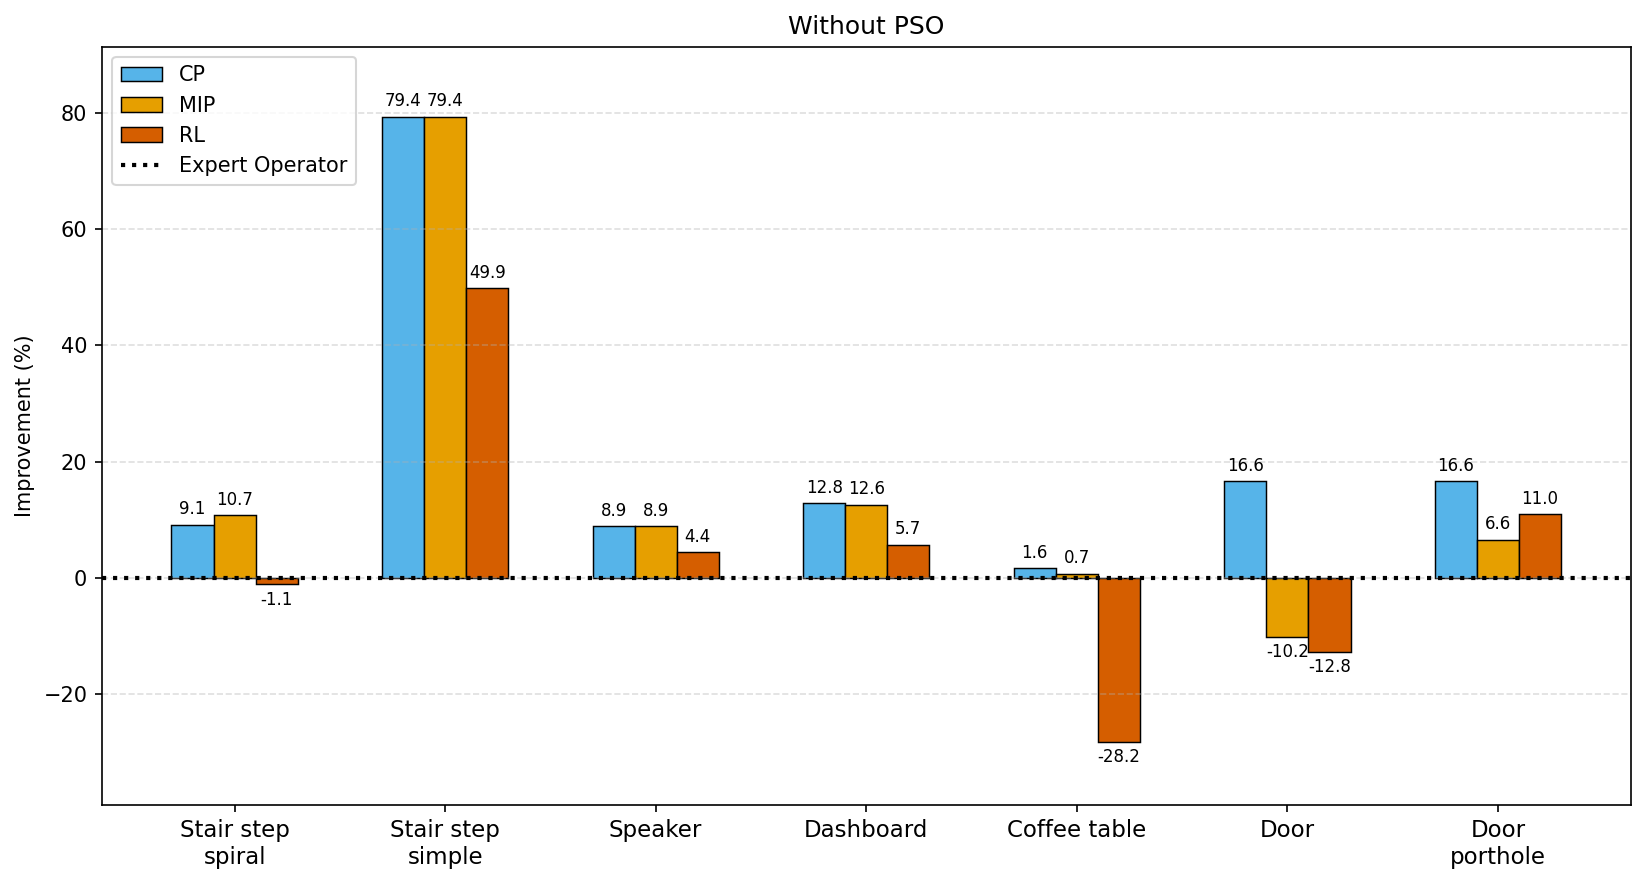
\includegraphics[width=0.7\textwidth]{img/comparison_plot_1.png}
		\caption{Percentage improvement over expert operator}
		\label{fig:comparison_plot1}
	\end{subfigure}
	%\hspace{1.5cm}
	\begin{subfigure}[b]{\textwidth}
		\centering
		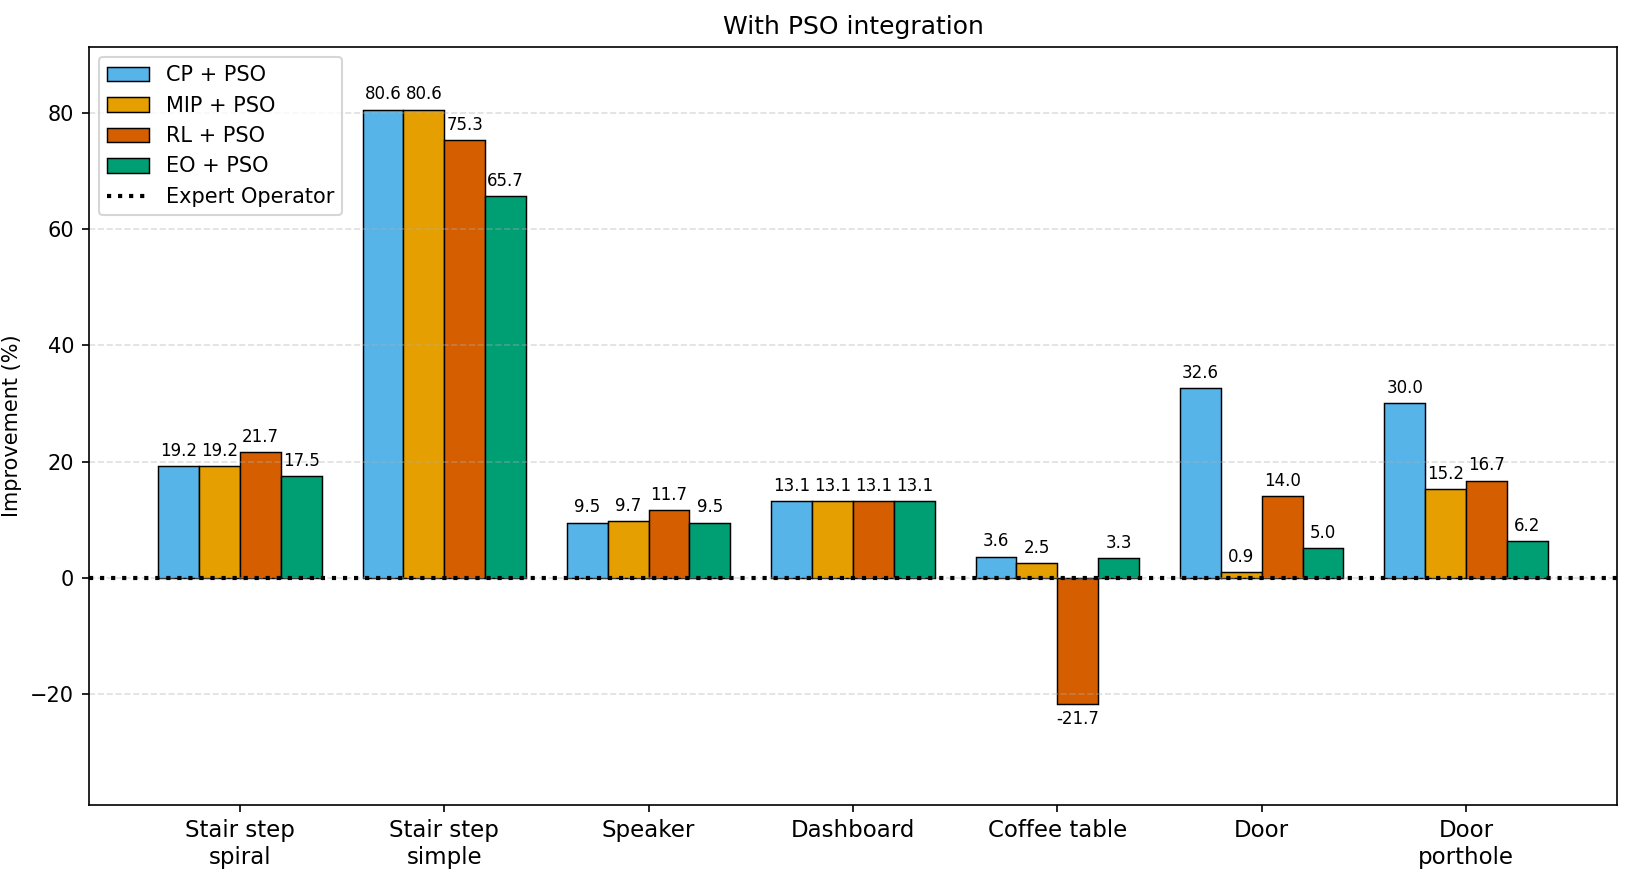
\includegraphics[width=0.7\textwidth]{img/comparison_plot_2.png}
		\caption{Percentage improvement over expert operator after PSO refinement}
		\label{fig:comparision_plot2}
	\end{subfigure}
	\caption{Percentage improvement relative to the solution provided by the expert operator. The first plot illustrates the improvements achieved by the CP model, MIP model and Q-learning algorithm without PSO integration, whereas the second plot presents the improvements obtained with PSO integration, alongside the improvement of the expert operator's solution when combined with PSO.}
	\label{fig:improvement}
\end{figure}

%\begin{figure}[t]
%	\centering
%	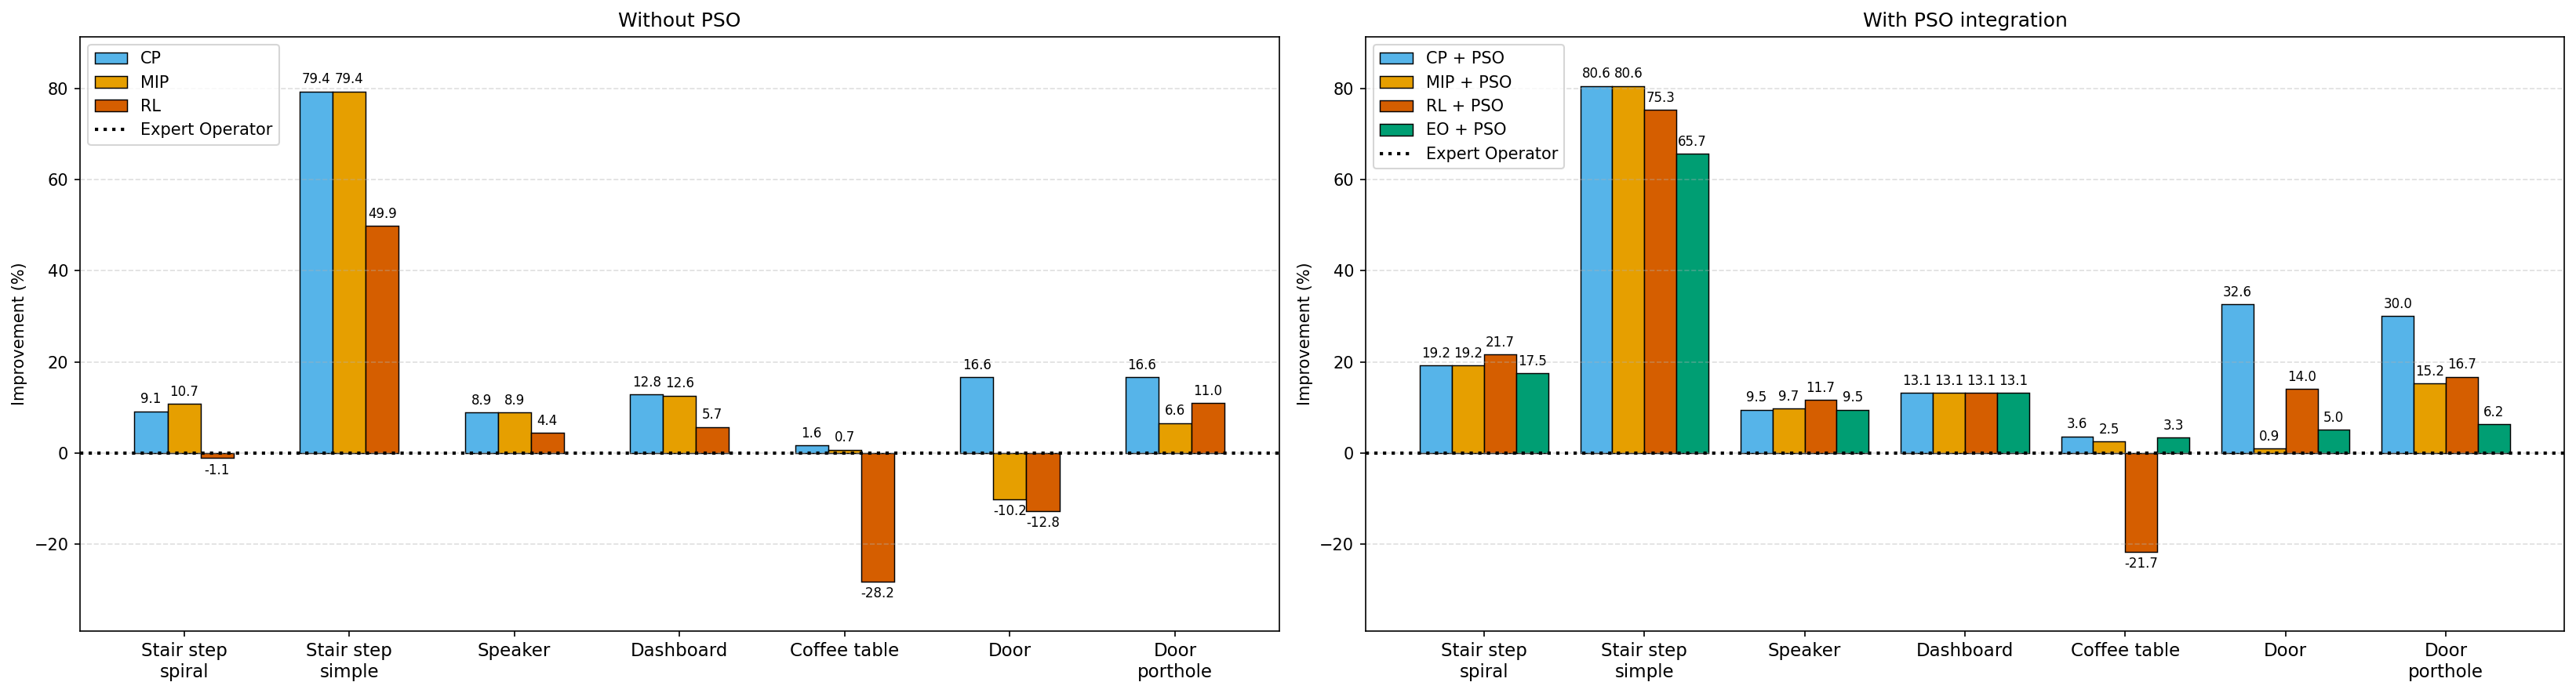
\includegraphics[width=\linewidth]{img/comparison_plot.png}
%	\caption{
%		Percentage improvement relative to the solution provided by the expert operator. The left plot illustrates the improvements achieved by the CP model, MIP model and Q-learning algorithm without PSO integration, whereas the right plot presents the improvements obtained with PSO integration, alongside the improvement of the expert operator's solution when combined with PSO.
%	}
%	\label{fig:improvement}
%\end{figure}

For each workpiece, the best CP and MIP solutions in terms of $\finer$, together with the Q-learning solution, were used as initial ones for the PSO algorithm. 

To enable direct integration into the target industrial system, the PSO algorithm was implemented in Java~18.0.2. Its hyper-parameters were tuned using the Optuna framework~\cite{akiba2019optuna}, yielding the following configuration: $\swarmsize = 1374$, $\maxiter = 2912$, $w = 0.669$, $c_1 = 2.385$, and $c_2 = 0.558$.

Figure~\ref{fig:improvement} shows the percentage improvement in $\finer$ with respect to the layout proposed by an expert operator. The first plot (Fig~\ref{fig:comparison_plot1}) reports the improvements achieved by the CP model, the MIP model, and the Q-learning algorithm before PSO refinement, whereas the second plot (Fig~\ref{fig:comparison_plot2}) shows the corresponding results after PSO refinement, including those obtained by initializing PSO from the expert layout.

The largest workpieces, namely the coffee table, the door, and the door with porthole, represent the most challenging instances. Among the considered approaches, the CP model consistently achieves the best improvements over the expert layout and is the only one that improves upon the expert solution for the door workpiece.

The Q-learning algorithm outperforms the expert layout in four of the seven considered workpieces. The integration with PSO further improves the solutions generated by the Q-learning algorithm for the stair step of the spiral staircase and the door, allowing them to surpass the expert layout. Conversely, starting from the Q-learning solution for the coffee table, only marginal improvements are obtained, highlighting the importance of starting the PSO search from a high-quality initial solution.

\begin{table}[!t]
	\centering
	\renewcommand{\arraystretch}{1.3}
	\setlength{\tabcolsep}{3pt}
	\caption{Summary of the best solutions, corresponding solution providers, and moment of inertia values for the different workpieces. 
		The workpiece perimeter is shown with solid lines. Dashed lines indicate extrusion areas, fixture regions are marked with diagonal hatching, and supporting bars are shown as shaded rectangles.}
	\label{tab:visual_results}
	\begin{tabular}{c c c c c}
		\hline
		\textbf{Workpiece} & \textbf{Expert Operator} & \textbf{Best CP/MIP} & \textbf{Q-learning} & \textbf{Best with PSO} \\
		\hline
		\makecell{Spiral stair step} & \makecell{$1.96057\times 10^{9}$ \\ 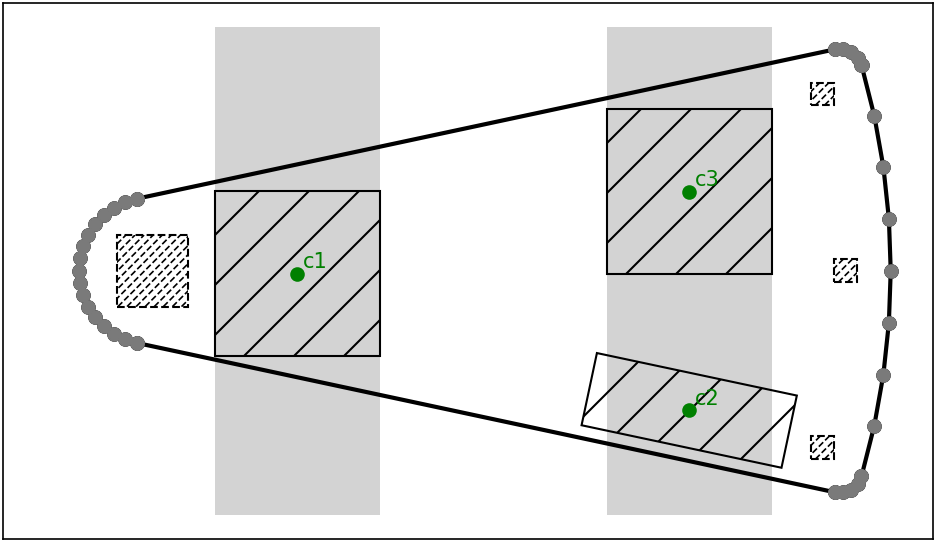
\includegraphics[width=0.18\linewidth]{img/spiral_stair_step_expert_operator.png}} & \makecell{MIP: $2.17089\times 10^{9}$ \\ 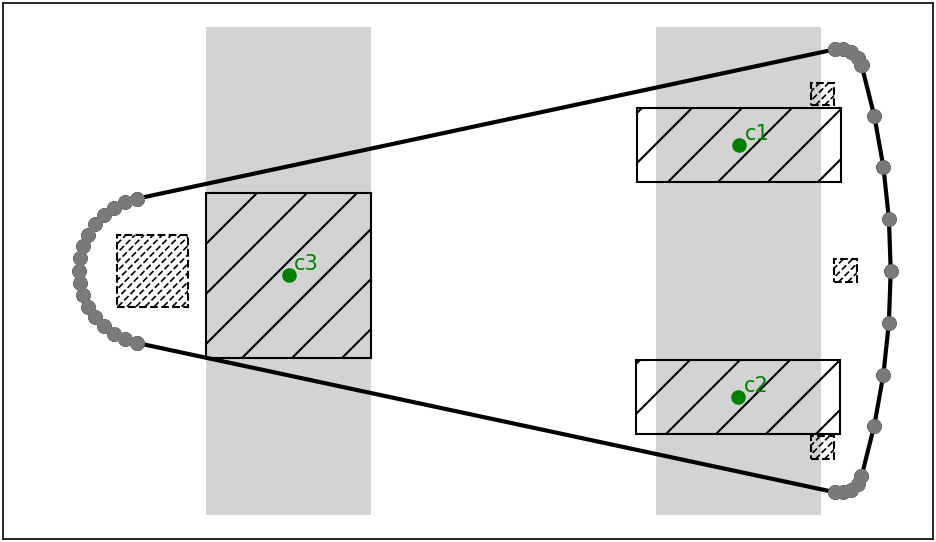
\includegraphics[width=0.18\linewidth]{img/spiral_stair_step_mip_model_gurobi.png}} & \makecell{$1.93822\times 10^{9}$ \\ 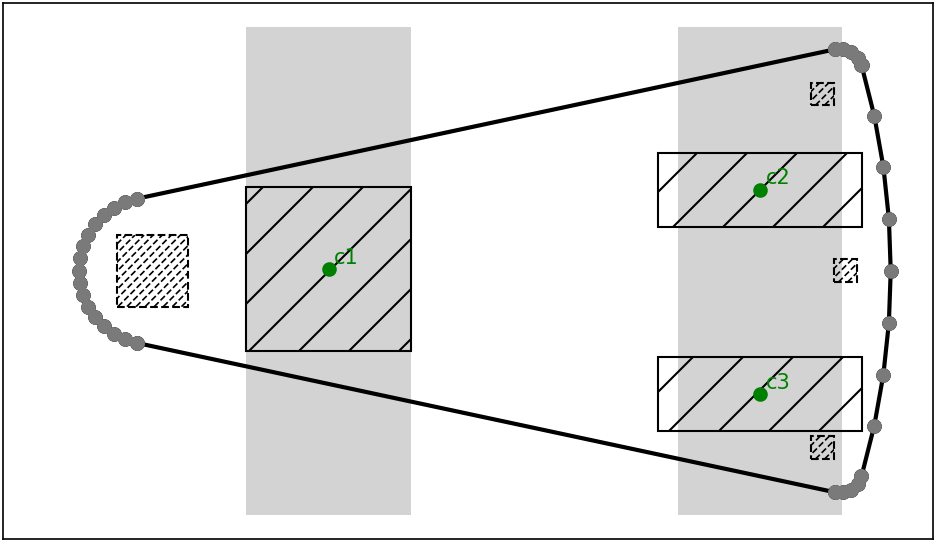
\includegraphics[width=0.18\linewidth]{img/spiral_stair_step_rl.png}} & \makecell{RL: $2.38520\times 10^{9}$ \\ 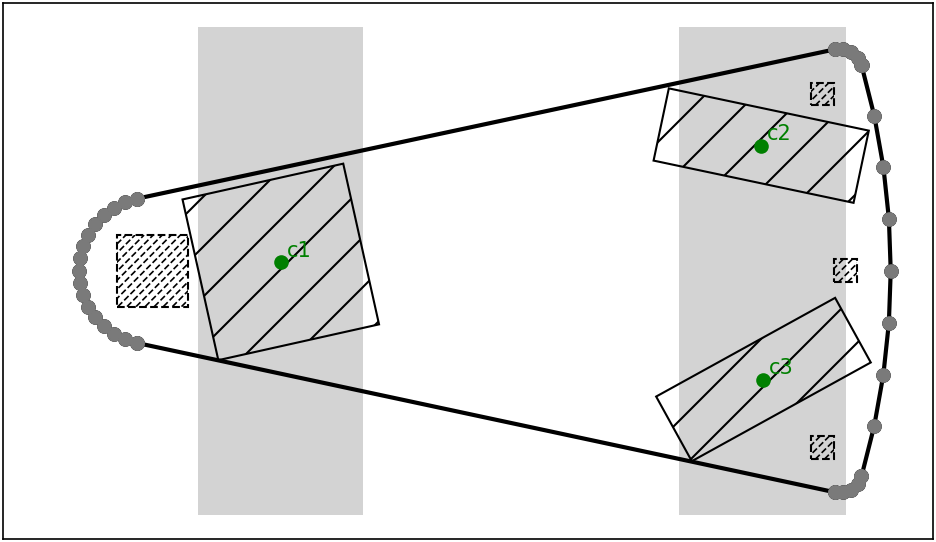
\includegraphics[width=0.18\linewidth]{img/spiral_stair_step_pso_rl_pso.png}} \\
		\hline
		\makecell{Simple stair step} & \makecell{$3.77213\times 10^{9}$ \\ 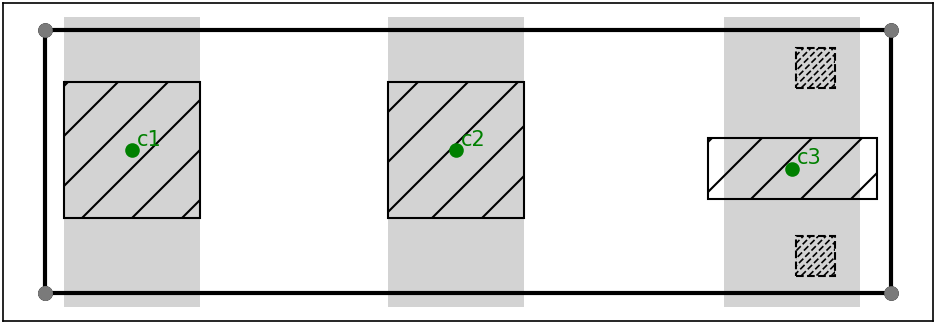
\includegraphics[width=0.18\linewidth]{img/simple_stair_step_expert_operator.png}} & \makecell{MIP: $6.76638\times 10^{9}$ \\ 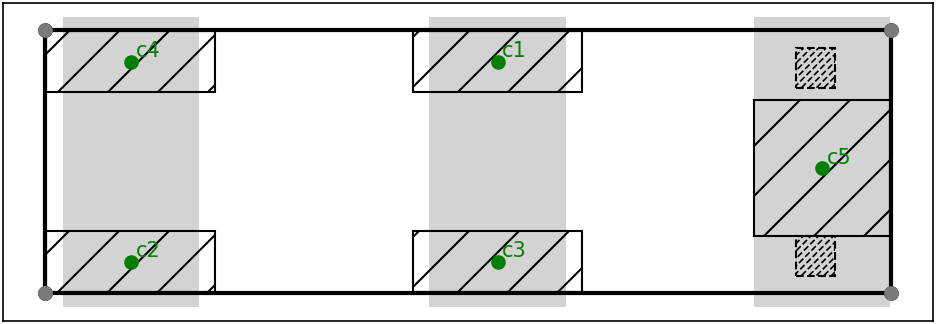
\includegraphics[width=0.18\linewidth]{img/simple_stair_step_mip_model_gurobi.png}} & \makecell{$5.65433\times 10^{9}$ \\ 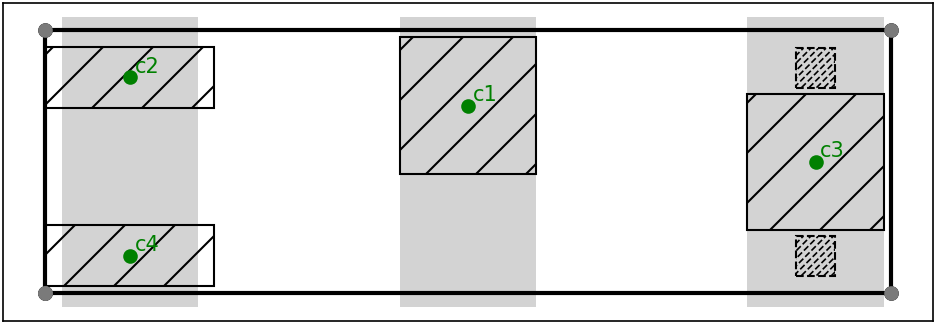
\includegraphics[width=0.18\linewidth]{img/simple_stair_step_rl.png}} & \makecell{CP: $6.81108\times 10^{9}$ \\ 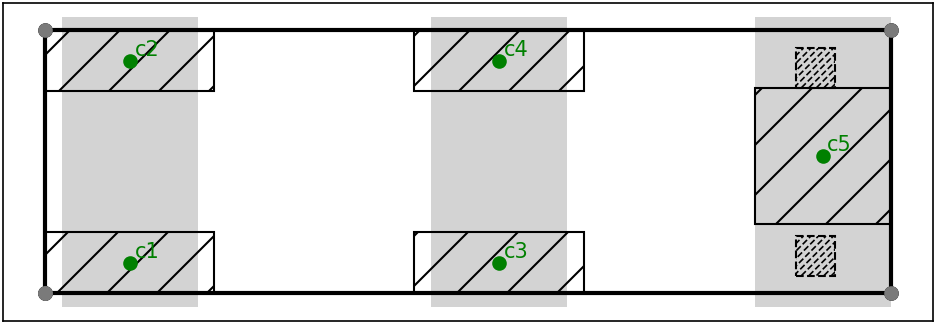
\includegraphics[width=0.18\linewidth]{img/simple_stair_step_pso_cp_pso.png}} \\
		\hline
		\makecell{Dashboard} & \makecell{$6.29544\times 10^{9}$ \\ 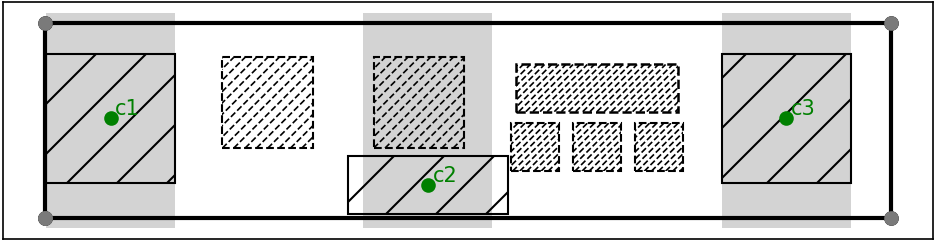
\includegraphics[width=0.18\linewidth]{img/dashboard_expert_operator.png}} & \makecell{CP: $7.10094\times 10^{9}$ \\ 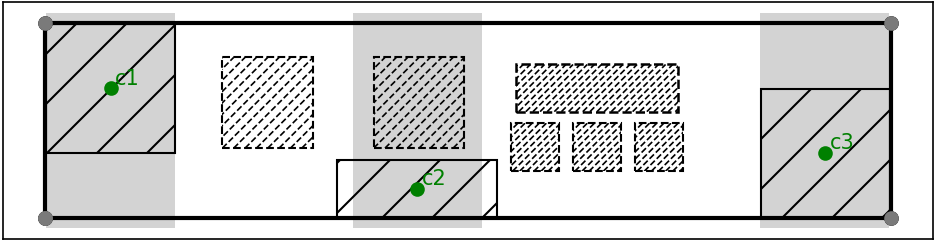
\includegraphics[width=0.18\linewidth]{img/dashboard_cp_model_gecode.png}} & \makecell{$6.65446\times 10^{9}$ \\ 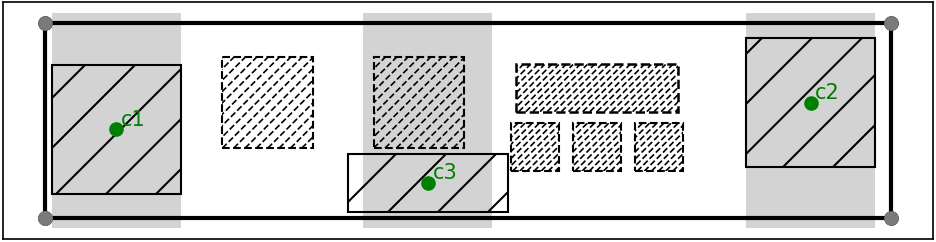
\includegraphics[width=0.18\linewidth]{img/dashboard_rl.png}} & \makecell{CP: $7.12226\times 10^{9}$ \\ 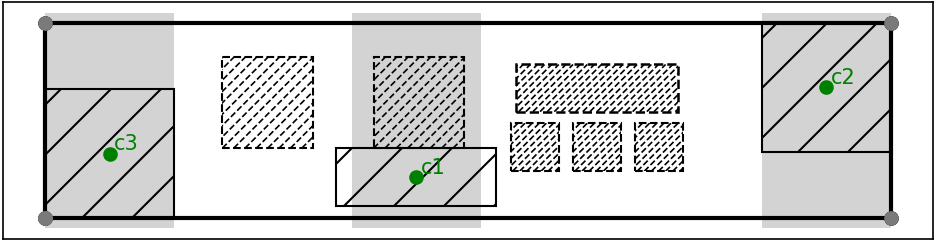
\includegraphics[width=0.18\linewidth]{img/dashboard_pso_cp_pso.png}} \\
		\hline
		\makecell{Speaker} & \makecell{$2.69490\times 10^{9}$ \\ 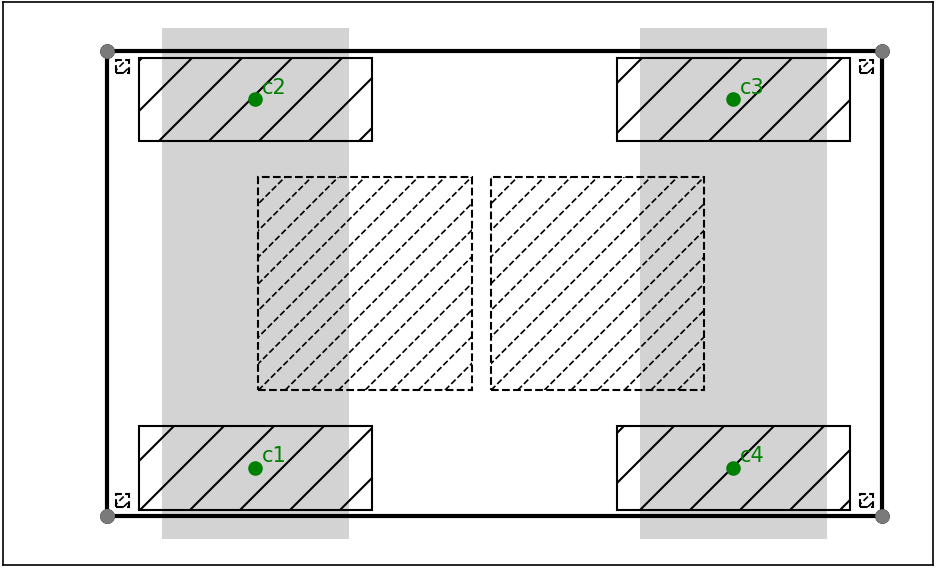
\includegraphics[width=0.18\linewidth]{img/speaker_expert_operator.png}} & \makecell{CP, MIP: $2.93433\times 10^{9}$ \\ 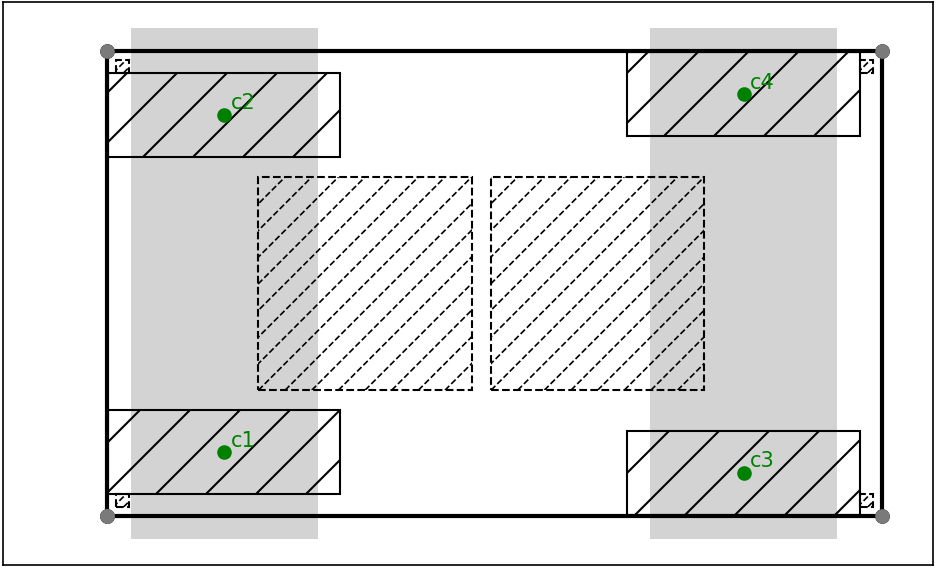
\includegraphics[width=0.18\linewidth]{img/speaker_cp_model_gecode.png}} & \makecell{$2.81248\times 10^{9}$ \\ 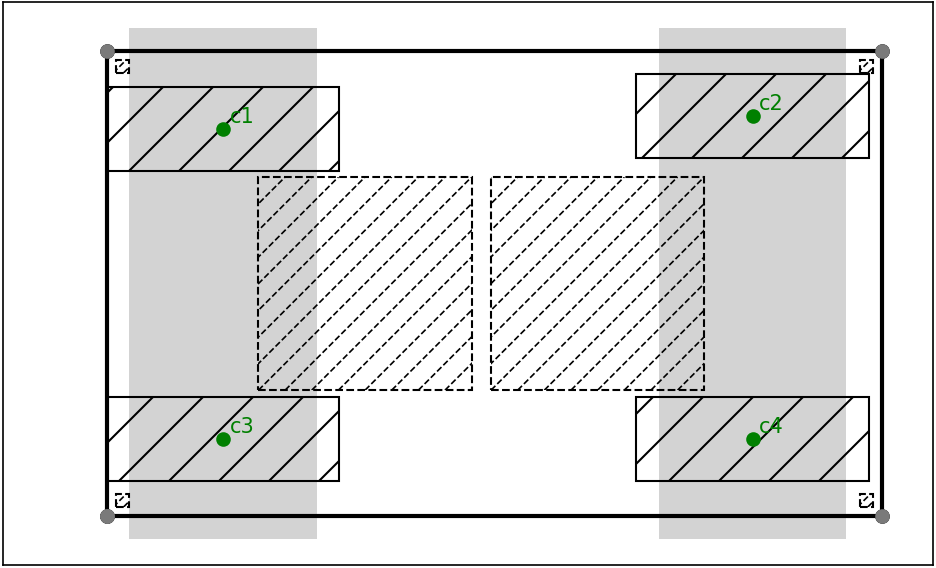
\includegraphics[width=0.18\linewidth]{img/speaker_rl.png}} & \makecell{RL: $3.00979\times 10^{9}$ \\ 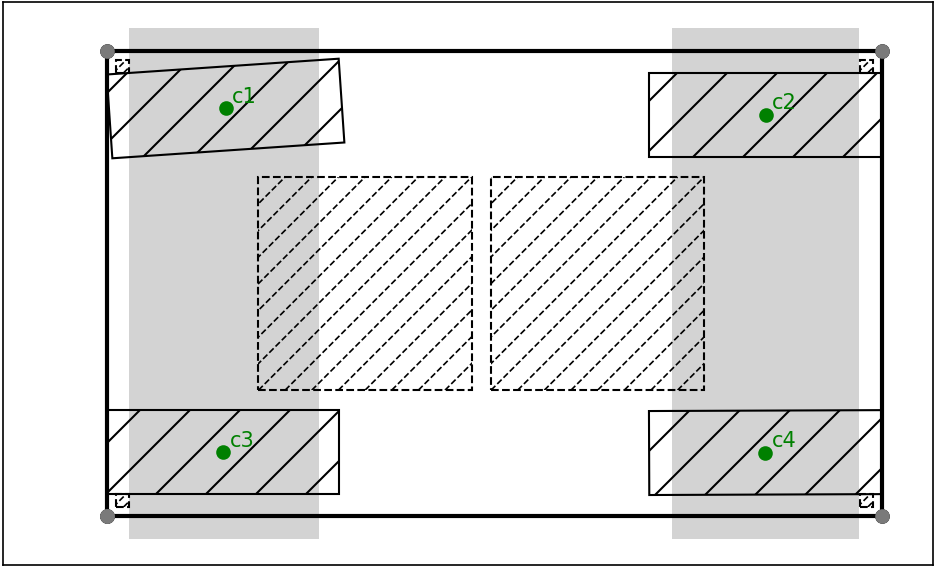
\includegraphics[width=0.18\linewidth]{img/speaker_pso_rl_pso.png}} \\
		\hline
		\makecell{Coffee table} & \makecell{$2.17954\times 10^{10}$ \\ 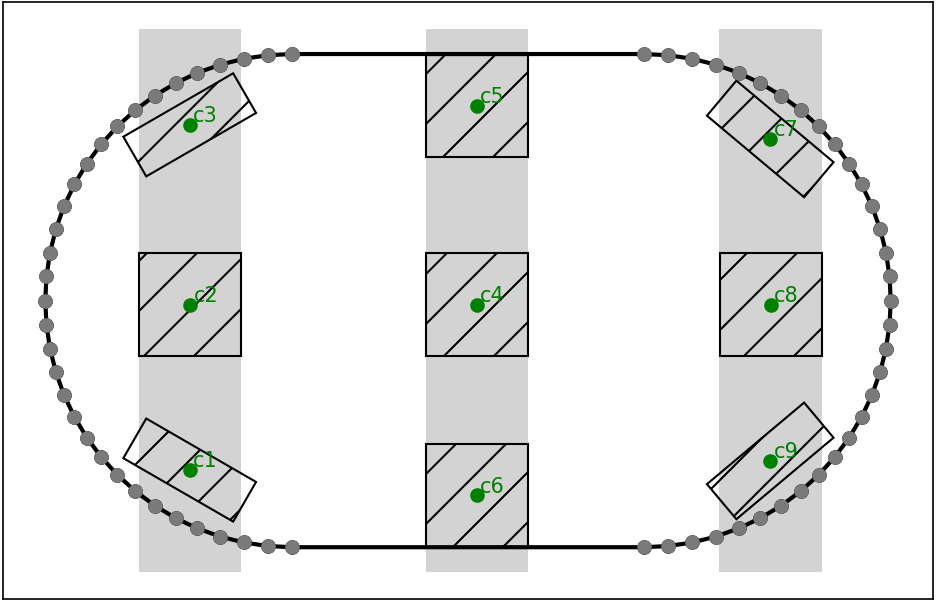
\includegraphics[width=0.18\linewidth]{img/coffee_table_expert_operator.png}} & \makecell{CP: $2.21449\times 10^{10}$ \\ 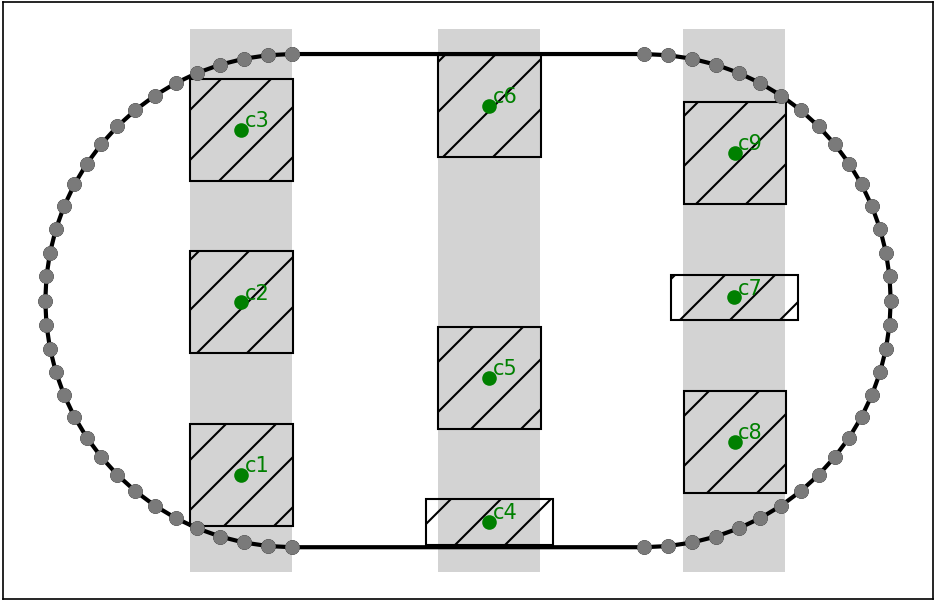
\includegraphics[width=0.18\linewidth]{img/coffee_table_cp_model_chuffed.png}} & \makecell{$1.56444\times 10^{10}$ \\ 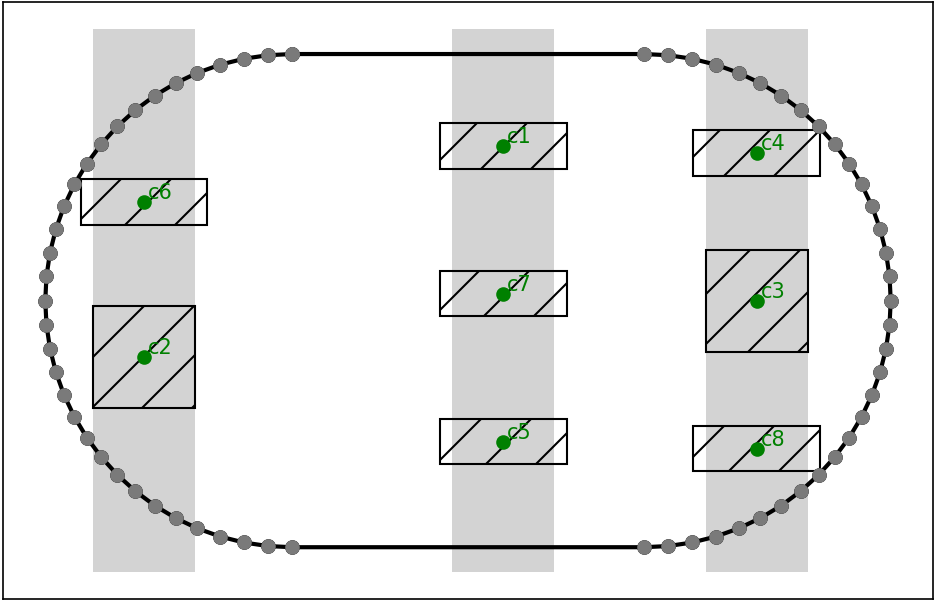
\includegraphics[width=0.18\linewidth]{img/coffee_table_rl.png}} & \makecell{CP: $2.25868\times 10^{10}$ \\ 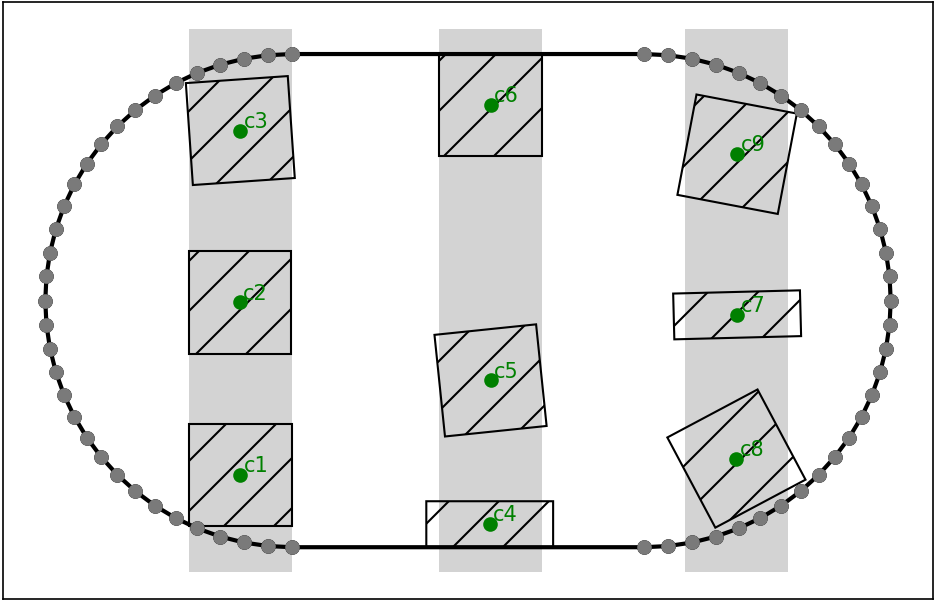
\includegraphics[width=0.18\linewidth]{img/coffee_table_pso_cp_pso.png}} \\
		\hline
		\makecell{Door} & \makecell{$1.31109\times 10^{11}$ \\ 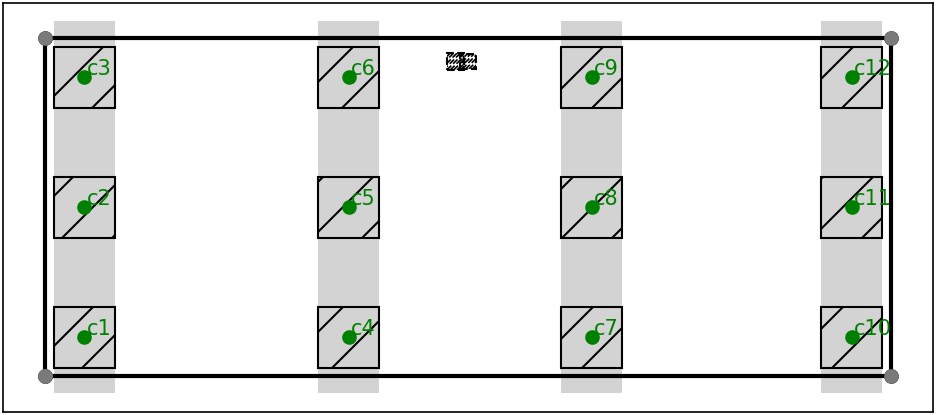
\includegraphics[width=0.18\linewidth]{img/door_expert_operator.png}} & \makecell{CP: $1.52925\times 10^{11}$ \\ 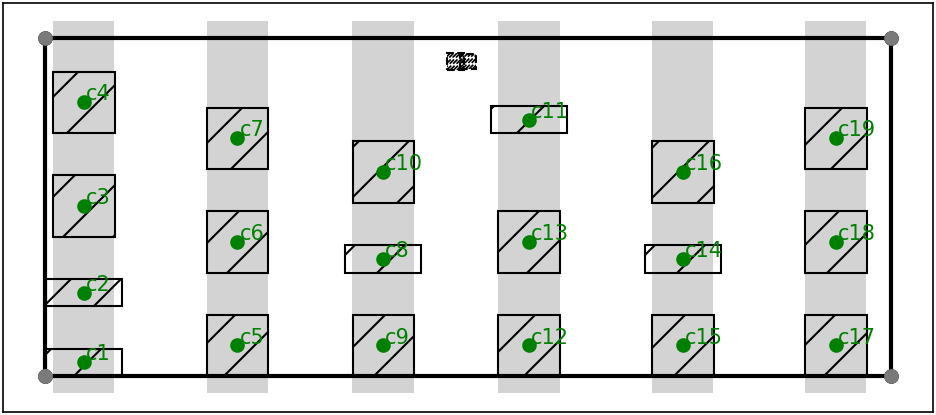
\includegraphics[width=0.18\linewidth]{img/door_LNS_cp_model_gecode.png}} & \makecell{$1.14387\times 10^{11}$ \\ 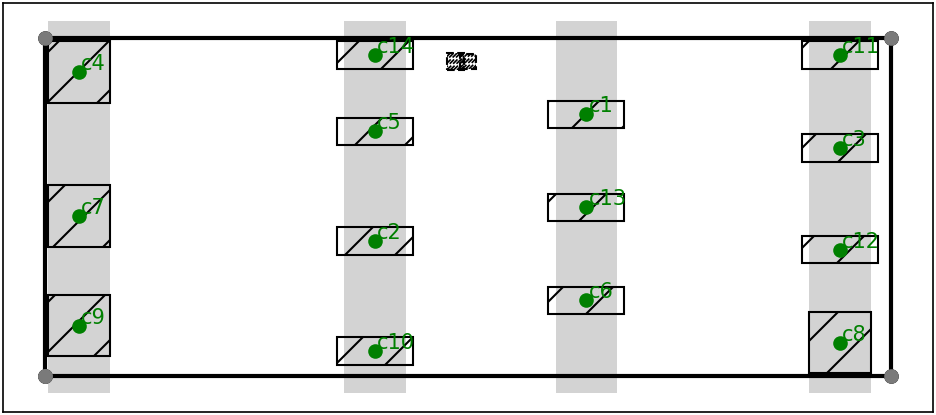
\includegraphics[width=0.18\linewidth]{img/door_rl.png}} & \makecell{CP: $1.73826\times 10^{11}$ \\ 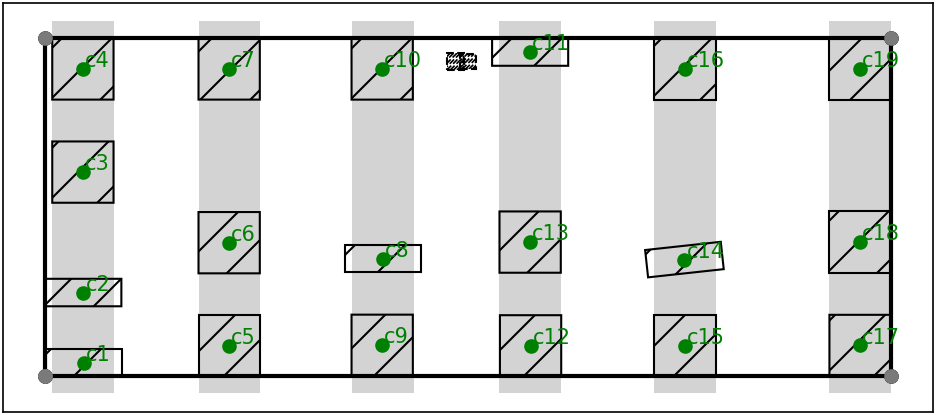
\includegraphics[width=0.18\linewidth]{img/door_pso_cp_pso.png}} \\
		\hline
		\makecell{Door porthole} & \makecell{$1.31109\times 10^{11}$ \\ 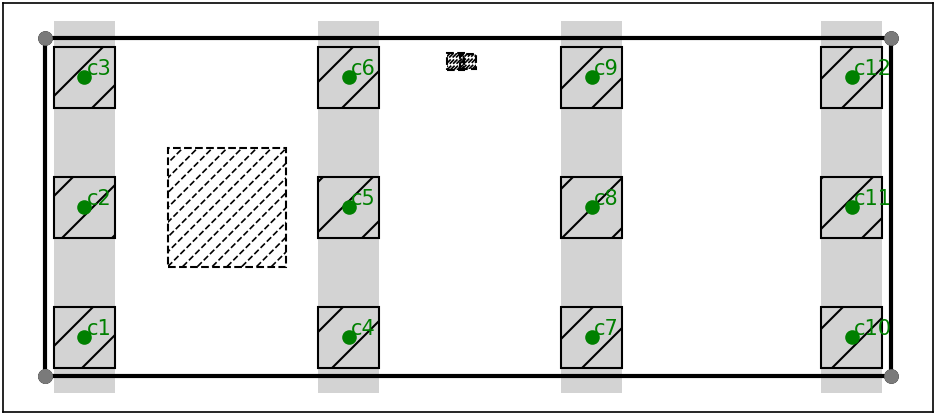
\includegraphics[width=0.18\linewidth]{img/door_porthole_expert_operator.png}} & \makecell{CP: $1.52861\times 10^{11}$ \\ 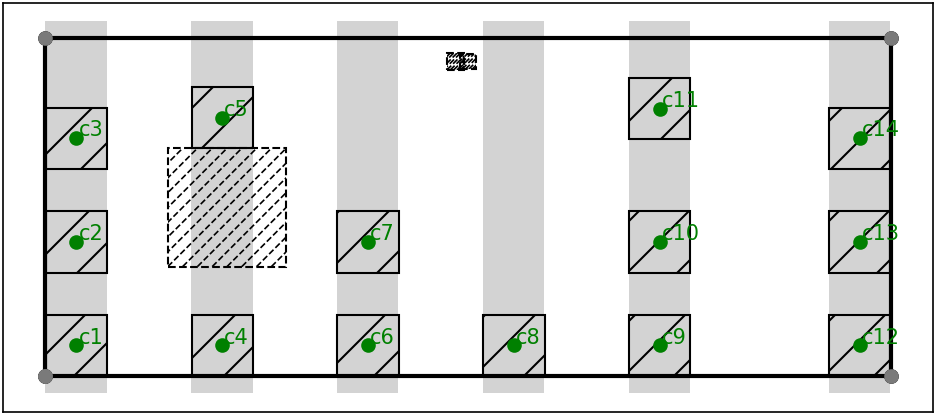
\includegraphics[width=0.18\linewidth]{img/door_porthole_LNS_cp_model_gecode.png}} & \makecell{$1.45467\times 10^{11}$ \\ 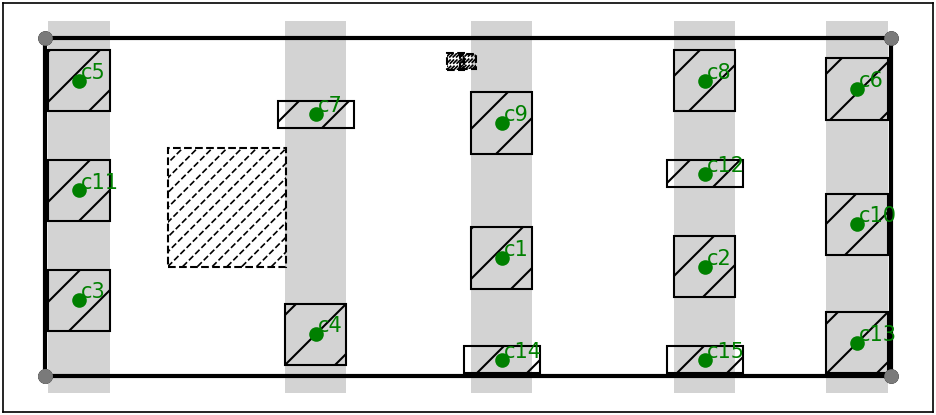
\includegraphics[width=0.18\linewidth]{img/door_porthole_rl.png}} & \makecell{CP: $1.70507\times 10^{11}$ \\ 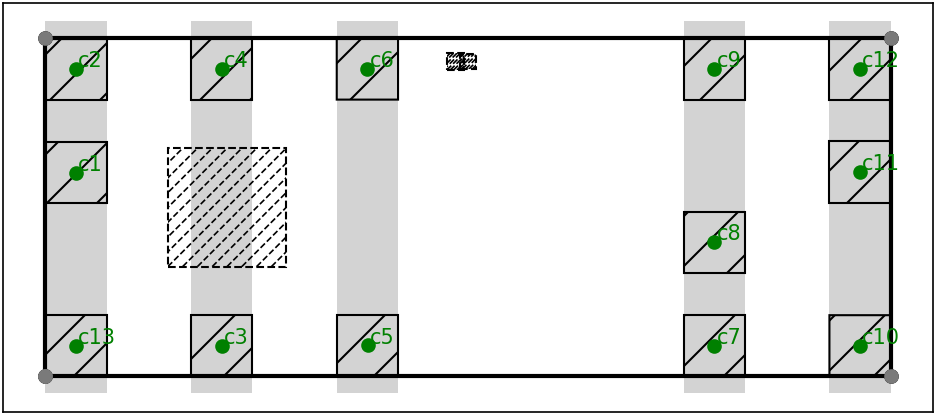
\includegraphics[width=0.18\linewidth]{img/door_porthole_pso_cp_pso.png}} \\
		\hline
	\end{tabular}
\end{table}


Table~\ref{tab:visual_results} reports visual comparisons of the best solutions obtained with the CP model, the MIP model, and the Q-learning algorithm for the different workpieces, together with the corresponding solutions refined by PSO. Note that, in the figures, the support bars can be positioned beneath the extrusion areas, since the fixture height prevents collisions between the cutting tools and the bars.

The layouts proposed by the Q-learning algorithm are qualitatively similar to those obtained with the CP and MIP models. An exception is the coffee table, where Q-learning tends to favour the placement of a larger number of rectangular fixtures instead of square ones, resulting in a lower value for the moment of inertia.

Rotation plays an important role in the stair step of the spiral staircase and coffee table workpieces, where fixture orientation improves adherence to the workpiece boundary. For the Speaker workpiece, the PSO refinement of the Q-learning solution introduces only a slight rotation of the upper-left fixture, yielding the marginal improvement reported in Figure~\ref{fig:improvement}.

The Stair step of the simple staircase exhibits the largest improvement over the expert layout. This is mainly due to the use of a larger number of fixtures, five for the CP and MIP models and four for the Q-learning algorithm, compared with the three fixtures used by the expert operator.

For both the door and the door with a porthole workpieces, the expert operator adopts a symmetric fixture layout, whereas the PSO refinement tends to move the fixtures farther from the workpiece centre. Since the principal moments of inertia are maximised when the fixtures are placed away from the symmetry axes, this configuration yields higher values of $\finer$. Moreover, in the door workpiece, the expert layout relies exclusively on square fixtures, whereas the optimization strategies increase the number of fixtures using even rectangular ones, thereby increasing the supported area of the workpiece.

Overall, the best trade-off between computational time and solution quality is achieved by integrating the CP model with PSO. Moreover, the CP formulation is expected to scale better to problems involving additional fixture types and multiple extrusion areas owing to the stronger propagation of the \texttt{diffn} global constraint and the fact that type and overlap decisions are modeled through discrete variables that cannot be relaxed, unlike the $x$ and $y$ variables in the MIP formulation.



\section{Conclusion}
\label{sec:conclusions}
This paper presented a comparative study of different solution strategies for the fixture layout optimization problem in wood industry.

The problem was first addressed through Constraint Programming (CP) and Mixed Integer Programming (MIP) models, whose performance was compared with that of a Q-learning-based algorithm. The experimental results showed that the CP formulation generally provides the best layouts in terms of the moment of inertia objective, with the $\lns$ solver consistently generating feasible solutions even for the most challenging instances, where other CP solvers fail.

Since the CP, MIP, and Q-learning approaches do not explicitly account for fixture rotations, their solutions were subsequently refined through a Particle Swarm Optimization (PSO) meta-heuristic, which treats fixture rotation as an additional decision variable, thereby addressing the complete optimization problem.

Among the considered approaches, the CP model refined by PSO provides the best trade-off between computational time and solution quality. Although the Q-learning algorithm does not always outperform the layouts proposed by the expert operator, its integration with PSO significantly improves the obtained solutions, surpassing the expert layouts for all the tested workpieces except the coffee table, for which the initial Q-learning solution was the weakest.

PSO also proves effective when initialized directly from the expert operator's layout, consistently improving the proposed solutions. This demonstrates its potential as a practical standalone refinement tool that can assist operators in further enhancing manually designed fixture layouts.

Future work may be focus on extending the proposed models to simultaneously optimize the fixture layouts of multiple workpieces on the machine worktable, as well as investigating alternative meta-heuristic and learning-based refinement strategies.



%% The Appendices part is started with the command \appendix;
%% appendix sections are then done as normal sections
%% \appendix

%% \section{}
%% \label{}

%% References
%%
%% Following citation commands can be used in the body text:
%% Usage of \cite is as follows:
%%   \cite{key}         ==>>  [#]
%%   \cite[chap. 2]{key} ==>> [#, chap. 2]
%%

%% References with BibTeX database:

\bibliographystyle{elsarticle-num}
\bibliography{bibliography}

%% Authors are advised to use a BibTeX database file for their reference list.
%% The provided style file elsarticle-num.bst formats references in the required Procedia style

%% For references without a BibTeX database:

% \begin{thebibliography}{00}

%% \bibitem must have the following form:
%%   \bibitem{key}...
%%

% \bibitem{}

% \end{thebibliography}

\end{document}

%%
%% End of file `ecrc-template.tex'. 